%%%%%%%%%%%%%%%%%%%%%%%%%%%%%%%%%%%%%%%%%%%%%%%%%%%
%% LaTeX book template                           %%
%% Author:  Amber Jain (http://amberj.devio.us/) %%
%% License: ISC license                          %%
%%%%%%%%%%%%%%%%%%%%%%%%%%%%%%%%%%%%%%%%%%%%%%%%%%%

\documentclass[a4paper,spanish,11pt]{book}
\usepackage[T1]{fontenc}
\usepackage[utf8]{inputenc}
\usepackage{lmodern}
%%%%%%%%%%%%%%%%%%%%%%%%%%%%%%%%%%%%%%%%%%%%%%%%%%%%%%%%%
% Source: http://en.wikibooks.org/wiki/LaTeX/Hyperlinks %
%%%%%%%%%%%%%%%%%%%%%%%%%%%%%%%%%%%%%%%%%%%%%%%%%%%%%%%%%
\usepackage{hyperref}
\usepackage{graphicx}
\usepackage[spanish]{babel}

%\usepackage[english]{babel}
%\usepackage[utf8]{inputenc}

\usepackage{pgf,tikz}

\usetikzlibrary{shapes, calc, shapes, arrows, math, babel, positioning}
\newcommand{\degre}{\ensuremath{^\circ}}
\usepackage{pgf,tikz,pgfplots}
\pgfplotsset{compat=1.15}
\usepackage{mathrsfs}
\usetikzlibrary{arrows}
%\pagestyle{empty}

\usepackage{amsmath,amssymb,textcomp, mathtools, adjustbox}
\everymath{\displaystyle}

\usepackage{graphicx}
\usepackage{xcolor}

\newcommand{\samedir}{\mathbin{\!/\mkern-5mu/\!}}

%%%%%%%%%%%%%%%%%%%%%%%%%%%%%%%%%%%%%%%%%%%%%%%%%%%%%%%%%%%%%%%%%%%%%%%%%%%%%%%%
% 'dedication' environment: To add a dedication paragraph at the start of book %
% Source: http://www.tug.org/pipermail/texhax/2010-June/015184.html            %
%%%%%%%%%%%%%%%%%%%%%%%%%%%%%%%%%%%%%%%%%%%%%%%%%%%%%%%%%%%%%%%%%%%%%%%%%%%%%%%%
\newenvironment{dedication}
{
   \cleardoublepage
   \thispagestyle{empty}
   \vspace*{\stretch{1}}
   \hfill\begin{minipage}[t]{0.66\textwidth}
   \raggedright
}
{
   \end{minipage}
   \vspace*{\stretch{3}}
   \clearpage
}

%%%%%%%%%%%%%%%%%%%%%%%%%%%%%%%%%%%%%%%%%%%%%%%%
% Chapter quote at the start of chapter        %
% Source: http://tex.stackexchange.com/a/53380 %
%%%%%%%%%%%%%%%%%%%%%%%%%%%%%%%%%%%%%%%%%%%%%%%%
\makeatletter
\renewcommand{\@chapapp}{}% Not necessary...
\newenvironment{chapquote}[2][2em]
  {\setlength{\@tempdima}{#1}%
   \def\chapquote@author{#2}%
   \parshape 1 \@tempdima \dimexpr\textwidth-2\@tempdima\relax%
   \itshape}
  {\par\normalfont\hfill--\ \chapquote@author\hspace*{\@tempdima}\par\bigskip}
\makeatother

%%%%%%%%%%%%%%%%%%%%%%%%%%%%%%%%%%%%%%%%%%%%%%%%%%%
% First page of book which contains 'stuff' like: %
%  - Book title, subtitle                         %
%  - Book author name                             %
%%%%%%%%%%%%%%%%%%%%%%%%%%%%%%%%%%%%%%%%%%%%%%%%%%%

% Book's title and subtitle
\title{\Huge \textbf{Mis apuntes}   \\\bigskip  \huge Compilación de apuntes de matemáticas \footnote{\url{https://github.com/crdguez/mis_mat_notas}}}
% Author
\author{\textsc{Carlos Rodríguez Jaso}\thanks{\url{https://crdguez.github.io/about/}}}
\date{}


\begin{document}

\frontmatter
\maketitle

%%%%%%%%%%%%%%%%%%%%%%%%%%%%%%%%%%%%%%%%%%%%%%%%%%%%%%%%%%%%%%%
% Add a dedication paragraph to dedicate your book to someone %
%%%%%%%%%%%%%%%%%%%%%%%%%%%%%%%%%%%%%%%%%%%%%%%%%%%%%%%%%%%%%%%
%\begin{dedication}
%Dedicated to Calvin and Hobbes.
%\end{dedication}

%%%%%%%%%%%%%%%%%%%%%%%%%%%%%%%%%%%%%%%%%%%%%%%%%%%%%%%%%%%%%%%%%%%%%%%%
% Auto-generated table of contents, list of figures and list of tables %
%%%%%%%%%%%%%%%%%%%%%%%%%%%%%%%%%%%%%%%%%%%%%%%%%%%%%%%%%%%%%%%%%%%%%%%%
\tableofcontents
%\listoffigures
%\listoftables

\mainmatter

%%%%%%%%%%%
% Preface %
%%%%%%%%%%%
%\chapter*{Preface}
%Lorem ipsum dolor sit amet, consectetur adipiscing elit. Duis risus ante, auctor et pulvinar non, posuere ac lacus. Praesent egestas nisi id metus rhoncus ac lobortis sem hendrerit. Etiam et sapien eget lectus interdum posuere sit amet ac urna.
%
%\section*{Un-numbered sample section}
%Lorem ipsum dolor sit amet, consectetur adipiscing elit. Duis risus ante, auctor et pulvinar non, posuere ac lacus. Praesent egestas nisi id metus rhoncus ac lobortis sem hendrerit. Etiam et sapien eget lectus interdum posuere sit amet ac urna. Aliquam pellentesque imperdiet erat, eget consectetur felis malesuada quis. Pellentesque sollicitudin, odio sed dapibus eleifend, magna sem luctus turpis.
%
%\section*{Another sample section}
%Lorem ipsum dolor sit amet, consectetur adipiscing elit. Duis risus ante, auctor et pulvinar non, posuere ac lacus. Praesent egestas nisi id metus rhoncus ac lobortis sem hendrerit. Etiam et sapien eget lectus interdum posuere sit amet ac urna. Aliquam pellentesque imperdiet erat, eget consectetur felis malesuada quis. Pellentesque sollicitudin, odio sed dapibus eleifend, magna sem luctus turpis, id aliquam felis dolor eu diam. Etiam ullamcorper, nunc a accumsan adipiscing, turpis odio bibendum erat, id convallis magna eros nec metus.
%
%\section*{Structure of book}
%% You might want to add short description about each chapter in this book.
%Each unit will focus on <SOMETHING>.
%
%\section*{About the companion website}
%The website\footnote{\url{https://github.com/amberj/latex-book-template}} for this file contains:
%\begin{itemize}
%  \item A link to (freely downlodable) latest version of this document.
%  \item Link to download LaTeX source for this document.
%  \item Miscellaneous material (e.g. suggested readings etc).
%\end{itemize}
%
%%%%%%%%%%%%%%%%%%%%%%%%%%%%%%%%%%%%%
%% Give credit where credit is due. %
%% Say thanks!                      %
%%%%%%%%%%%%%%%%%%%%%%%%%%%%%%%%%%%%%
%\section*{Acknowledgements}
%\begin{itemize}
%\item A special word of thanks goes to Professor Don Knuth\footnote{\url{http://www-cs-faculty.stanford.edu/~uno/}} (for \TeX{}) and Leslie Lamport\footnote{\url{http://www.lamport.org/}} (for \LaTeX{}).
%\item I'll also like to thank Gummi\footnote{\url{http://gummi.midnightcoding.org/}} developers and LaTeXila\footnote{\url{http://projects.gnome.org/latexila/}} development team for their awesome \LaTeX{} editors.
%\item I'm deeply indebted my parents, colleagues and friends for their support and encouragement.
%\end{itemize}
%\mbox{}\\
%%\mbox{}\\
%\noindent Amber Jain \\
%\noindent \url{http://amberj.devio.us/}

%%%%%%%%%%%%%%%%
% NEW CHAPTER! %
%%%%%%%%%%%%%%%%
%\part{Matemáticas de 4ºESO}

\chapter{Geometría}

\definecolor{wrwrwr}{rgb}{0.3803921568627451,0.3803921568627451,0.3803921568627451}
\definecolor{rvwvcq}{rgb}{0.98235294117647059,0.396078431372549,0.7529411764705882}
%
%
%
%\begin{tikzpicture}[grow=right, sloped, scale=0.7]\clip(-6.154568000000002,-3.8982211062725844) rectangle (4.2,7);
%\clip(-11.145015598814782,-9.076966577456616) rectangle (18.28831648795786,8.422371196936597);
%\fill[line width=2pt,color=red,fill=rvwvcq,fill opacity=0.00000000149011612] (-5,-1) -- (3,-1) -- (0,6) -- cycle;
%\draw[line width=1.6pt,fill=black,fill opacity=0.10000000149011612] (-2.616480014189626,2.336927980134524) -- (-2.1696242105403662,2.0177452632421953) -- (-1.8504414936480373,2.464601066891455) -- (-2.2972972972972974,2.7837837837837838) -- cycle; 
%\draw[line width=1.6pt,fill=black,fill opacity=0.10000000149011612] (1.5423027784864105,2.401293516865042) -- (1.0375609857592993,2.1849756056962804) -- (1.2538788969280612,1.6802338129691692) -- (1.7586206896551724,1.896551724137931) -- cycle; 
%\draw[line width=1.6pt,fill=black,fill opacity=0.10000000149011612] (0.5491427100652383,-1) -- (0.5491427100652384,-0.4508572899347618) -- (0,-0.4508572899347617) -- (0,-1) -- cycle; 
%\draw [line width=2pt,color=rvwvcq] (-5,-1)-- (3,-1);
%\draw [line width=2pt,color=rvwvcq] (3,-1)-- (0,6);
%\draw [line width=2pt,color=rvwvcq] (0,6)-- (-5,-1);
%\draw [line width=2pt,color=wrwrwr] (0,-9.076966577456616) -- (0,8.422371196936597);
%\draw [line width=2pt,color=wrwrwr,domain=-11.145015598814782:18.28831648795786] plot(\x,{(-8-3*\x)/-7});
%\draw [line width=2pt,color=wrwrwr,domain=-11.145015598814782:18.28831648795786] plot(\x,{(--8-5*\x)/7});
%\begin{scriptsize}
%\draw [fill=rvwvcq] (-5,-1) circle (2.5pt);
%\draw[color=rvwvcq] (-4.802740874752074,-0.42299719371372185) node {$A$};
%\draw [fill=rvwvcq] (3,-1) circle (2.5pt);
%\draw[color=rvwvcq] (3.1962913282494623,-0.42299719371372185) node {$B$};
%\draw [fill=rvwvcq] (0,6) circle (2.5pt);
%\draw[color=rvwvcq] (0.21930523328125284,6.576737916043563) node {$C$};
%\draw[color=black] (-1.0750365471397076,2.530016055715133) node {$\alpha = 90\textrm{\degre}$};
%\draw[color=black] (2.3937994243884666,2.256588902990239) node {$\beta = 90\textrm{\degre}$};
%\draw[color=black] (1.4877601780937941,-0.4776826242587007) node {$\gamma = 90\textrm{\degre}$};
%\draw [fill=wrwrwr] (0,1.1428571428571428) circle (2pt);
%\draw[color=wrwrwr] (1.8501758766116632,1.1355375768181737) node {$Ortocentro$};
%\end{scriptsize}
%\end{tikzpicture}
%
%\begin{tikzpicture}[line cap=round,line join=round,>=triangle 45,x=1cm,y=1cm, scale=0.8]
%\draw [color=lightgray,dash pattern=on 1pt off 1pt, xstep=1cm,ystep=1cm] (-0.6129302567150502,-0.43158220601634095) grid (9.010648940148005,6.1);
%\draw[->,color=black] (-0.6129302567150502,0) -- (9.010648940148005,0);
%\foreach \x in {,1,2,3,4,5,6,7,8,9}
%\draw[shift={(\x,0)},color=black] (0pt,2pt) -- (0pt,-2pt) node[below] {\footnotesize $\x$};
%\draw[->,color=black] (0,-0.43158220601634095) -- (0,6.1);
%\foreach \y in {,1,2,3,4,5,6}
%\draw[shift={(0,\y)},color=black] (2pt,0pt) -- (-2pt,0pt) node[left] {\footnotesize $\y$};
%\draw[color=black] (0pt,-10pt) node[right] {\footnotesize $0$};
%\clip(-0.6129302567150502,-0.43158220601634095) rectangle (9.010648940148005,7.8783927087822985);
%\draw [->,line width=1.5pt,color=red] (1,1) -- node[above,fill=white]{$\overrightarrow{v}=\left(6,4 \right) \land \left|\overrightarrow{v}\right|=\sqrt{6^2+4^2}=\sqrt{52}$} (7,5);
%\draw [-,line width=2pt,color=blue] (1,1) -- node[below]{$7-1=6$} (7,1);
%\draw [-,line width=2pt,color=orange] (7,1) -- node[right]{$5-1=4$}(7,5);
%
%\draw [fill=yellow, color=blue]  (1,1) circle (2pt) node[above] {$A = (1, 1)$};
%\draw [fill=yellow, color=blue]  (7,5) circle (2pt) node[above] {$B = (7, 5)$};
%\end{tikzpicture}
%%% Añade al preámbulo:
%\newcommand{\samedir}{\mathbin{\!/\mkern-5mu/\!}}


\section{Vectores Libres}

Dados dos puntos en el plano (A y B), podemos trazar  una flecha que vaya del primero al segundo. A esta flecha la llamaremos vector (fijo) y se denota $\overrightarrow{AB}$.



\begin{tikzpicture}[scale=0.75]
\coordinate (A) at (1,2);
\coordinate (B) at (6,4);

\draw [fill=blue] (A) circle (2pt) node [left] {A};
\draw [fill=blue] (B) circle (2pt) node [left] {B};

\draw [->, red, thick]  (A) -- node[below] {$\overrightarrow{AB}$} (B); 
\end{tikzpicture}




\begin{itemize}
\item \textbf{Módulo}: La longitud del vector
\item \textbf{Dirección}: La recta que contiene al vector y cualquiera de sus paralelas
\item \textbf{Sentido}: El que va del origen al final o su contrario. Viene representado por punta "la cabeza de la flecha"
\end{itemize}
Dos vectores (fijos) son \textbf{equipolentes} cuando tienen el mismo módulo, misma dirección y mismo sentido. Un vector fijo y todos sus equipolentes forman lo que de denomina un \textbf{vector libre}. Se denota $\overrightarrow{v}$ o $\left[\overrightarrow{AB}\right]$ siendo $\overrightarrow{AB}$ un vector fijo representante de $\overrightarrow{v}$. Un vector libre viene determinado por sus coordenadas:

\section{Coordenadas y módulo de un vector} Un vector se puede ver como el desplazamiento que tenemos que hacer horizontalmente y verticalmente para ir del origen al extremo del mismo. Al desplazamiento horizontal le llamaremos primera coordenada y al vertical, segunda.

\begin{itemize}
\item Dados $A(x_1,y_2),B(x_2,y_2) \to  \overrightarrow{AB}(x_2-x_1,y_2-y_1)$
\item A partir de las coordenadas del punto podremos calcular su módulo. Dados $\overrightarrow{u}(x,y), \to  \left|\overrightarrow{u}\right|=\sqrt{x^2+y^2}$
\end{itemize}




\subsection{Ejemplo}

Determina las coordenadas y el módulo del vector libre cuyo representante es el vector que va de $A(1,1)$ a $B(7,5)$

\begin{tikzpicture}[line cap=round,line join=round,>=triangle 45,x=1cm,y=1cm, scale=0.8]
\draw [color=lightgray,dash pattern=on 1pt off 1pt, xstep=1cm,ystep=1cm] (-0.6129302567150502,-0.43158220601634095) grid (9.010648940148005,6.1);
\draw[->,color=black] (-0.6129302567150502,0) -- (9.010648940148005,0);
\foreach \x in {,1,2,3,4,5,6,7,8,9}
\draw[shift={(\x,0)},color=black] (0pt,2pt) -- (0pt,-2pt) node[below] {\footnotesize $\x$};
\draw[->,color=black] (0,-0.43158220601634095) -- (0,6.1);
\foreach \y in {,1,2,3,4,5,6}
\draw[shift={(0,\y)},color=black] (2pt,0pt) -- (-2pt,0pt) node[left] {\footnotesize $\y$};
\draw[color=black] (0pt,-10pt) node[right] {\footnotesize $0$};
\clip(-0.6129302567150502,-0.43158220601634095) rectangle (9.010648940148005,7.8783927087822985);
\draw [->,line width=1.5pt,color=red] (1,1) -- node[above,fill=white]{$\overrightarrow{v}=\left(6,4 \right) \land \left|\overrightarrow{v}\right|=\sqrt{6^2+4^2}=\sqrt{52}$} (7,5);
\draw [-,line width=2pt,color=blue] (1,1) -- node[below]{$7-1=6$} (7,1);
\draw [-,line width=2pt,color=orange] (7,1) -- node[right]{$5-1=4$}(7,5);

\draw [fill=yellow, color=blue]  (1,1) circle (2pt) node[above] {$A = (1, 1)$};
\draw [fill=yellow, color=blue]  (7,5) circle (2pt) node[above] {$B = (7, 5)$};
\end{tikzpicture}



\section{Operaciones con vectores}
\subsection{Producto de un número por un vector}
\paragraph*{Definición}
Dado $k \in \mathbb{R}$ y $\overrightarrow{u}$ se define $k\cdot\overrightarrow{u}$ como un $\overrightarrow{v}$ que:\begin{itemize}
\item $\left|\overrightarrow{v}\right|=\left|k\right|\cdot\left|\overrightarrow{u}\right|$
\item $ \overrightarrow{v}\samedir\overrightarrow{u}$
\item Mismo sentido que $\overrightarrow{u}$ si $k>0$ o sentido contrario si $k>0$
\end{itemize}Además se cumple que si $\overrightarrow{u}(x_1,y_1)\to k\overrightarrow{u}(k\cdot x_1,k\cdot y_1)$

\subsubsection{Ejemplos}\begin{tikzpicture}[scale=0.75]
\draw [->, red, thick, fill=red]  (1,1) -- node[left] {$\overrightarrow{u}(1,2)$} (2,3); 
\draw [->, blue, thick, fill=blue]  (2,-1) -- node[left] {$2\overrightarrow{u}(2,4)$} (4,3); 
\draw [->, gray, thick, fill=blue]  (6,1) -- node[left] {$\frac{1}{2}\overrightarrow{u}(0.5,1)$} (6.5,2); 
\draw [->, orange, thick, fill=blue]  (8,3) -- node[right] {$-\frac{3}{2}\overrightarrow{u}(1.5,3)$} (6.5,0); 
\end{tikzpicture}

\subsection{Suma y resta de vectores}
\paragraph*{Definición de suma} Dados $\overrightarrow{u}$ y $\overrightarrow{v}$ se define la suma como el vector que   si los ponemos seguidos va del origen del primer vector al extremo del segundo vector. Además se cumple que si $\overrightarrow{u}(x_1,y_1) \ y \overrightarrow{v}(x_2,y_2) \to \overrightarrow{u} +\overrightarrow{v}(x_1+x_2, y_1+y_2)$ 
\medskip 

\begin{tikzpicture}[scale=0.75]
\draw [->, red, thick, fill=red]  (1,0) -- node[left] {$\overrightarrow{u}(1,2)$} (2,2); 
\draw [->, blue, thick, fill=blue]  (2,2) -- node[left] {$\overrightarrow{v}(4,1)$} (6,3); 
\draw [->, orange, thick, fill=blue]  (1,0) -- node[right] {$\overrightarrow{u}+\overrightarrow{v}(5,3)$} (6,3); 
\end{tikzpicture}

\paragraph*{Definición de resta} Dados $\overrightarrow{u}$ y $\overrightarrow{v}$ se define la resta como la suma del primero con el opuesto del segundo. Además se cumple que si $\overrightarrow{u}(x_1,y_1) \ y \overrightarrow{v}(x_2,y_2) \to \overrightarrow{u} -\overrightarrow{v}(x_1-x_2, y_1-y_2)$ 

\section{Punto medio de un segmento}

Dados dos puntos del plano, $A(x_1,y_1)$ y $B(x_2,y_2)$, el punto medio es $M(\frac{x_1+x_2}{2},\frac{y_1+y_2}{2})$. 

\begin{tikzpicture}[scale=0.75]

\tikzmath{\x1 = 1; \y1 =2;
		  \x2 = 6; \y2 =4; 	 
                   %computations are also possible
                    \x3 = (\x1 + \x2)*0.5; \y3 =(\y1 + \y2)*0.5; } 

\coordinate (A) at (\x1,\y1);
\coordinate (M) at (\x3,\y3);
\coordinate (B) at (\x2,\y2);

\draw [fill=blue] (A) circle (2pt) node [left] {$A(x_1,y_1)$};
\draw [fill=blue] (B) circle (2pt) node [right] {$B(x_2,y_2)$};
\draw [fill=blue] (M) circle (2pt) node [above] {$M(\frac{x_1+x_2}{2},\frac{y_1+y_2}{2})$};
\draw [->, red, thick]  (A) -- node[below] {$\overrightarrow{AB}$} (B); 

\end{tikzpicture}

La demostración es sencilla aplicando la propiedad geométrica que cumple el punto medio: $\overrightarrow{AM}=\overrightarrow{MB}$

\subsection{Ejemplo}
\begin{tikzpicture}[scale=0.5]

\tikzmath{\x1 = 1; \y1 = 4;
		  \x2 = 9; \y2 = 0; 	 
                   %computations are also possible
                    \x3 = (\x1 + \x2)*0.5; \y3 =(\y1 + \y2)*0.5; } 

\coordinate (A) at (\x1,\y1);
\coordinate (M) at (\x3,\y3);
\coordinate (B) at (\x2,\y2);

\draw [fill=blue] (A) circle (2pt) node [left] {A(\x1,\y1)};
\draw [fill=blue] (B) circle (2pt) node [right] {B(\x2,\y2)};
\draw [fill=blue] (M) circle (2pt) node [above] {M(\x3,\y3)};
\draw [->, red, thick]  (A) -- node[below] {$\overrightarrow{AB}$} (B); 

\end{tikzpicture}

\section{Puntos alineados}
Dados los puntos $A$, $B$ y $C$ estarán alineados si los vectores $\overrightarrow{AB}$ y $\overrightarrow{BC}$ son colineales, o tienen la misma dirección, y por tanto:
$\exists k\in\mathbb{R} | \ \left[\overrightarrow{BC}\right]=k\cdot\left[\overrightarrow{AB}\right]$

\begin{tikzpicture}[scale=0.75]

\tikzmath{\x1 = 1; \y1 =1;
		  \x2 = 3; \y2 =2;
		  \k=2; 	 
                   %computations are also possible
                    \x3 = \x2+(\x2 - \x1)*\k; \y3 =\y2+(\y2 - \y1)*\k; } 

\coordinate (A) at (\x1,\y1);
\coordinate (C) at (\x3,\y3);
\coordinate (B) at (\x2,\y2);

\draw [fill=blue] (A) circle (2pt) node [left] {A};
\draw [fill=blue] (B) circle (2pt) node [above] {B};
\draw [fill=blue] (C) circle (2pt) node [right] {C};
\draw [->, red, thick]  (A) -- node[below] {$\overrightarrow{AB}$} (B); 
\draw [->, red, thick]  (B) -- node[below, fill=white] {$\left[\overrightarrow{BC}\right]=k\cdot\left[\overrightarrow{AB}\right]$} (C); 

\end{tikzpicture}

o bien:

Si $\left[\overrightarrow{AB}\right]=\overrightarrow{u}(u1,u2)$ y  $\left[\overrightarrow{BC}\right]=\overrightarrow{v}(v1,v2)$, se cumple: $$\dfrac{v1}{u1}=\dfrac{v2}{u2}$$

\subsection{Ejemplo}
\begin{tikzpicture}[scale=0.75]

\tikzmath{\x1 = 1; \y1 =6;
		  \x2 = 2; \y2 =5.5;
		  \k=3; 	 
          %computations are also possible
          \x3 = \x2+(\x2 - \x1)*\k; \y3 =\y2+(\y2 - \y1)*\k;
          \u1 = \x2 - \x1; \u2 = \y2 - \y1;
          \v1 = \x3 - \x2; \v2 = \y3 - \y2; } 

\coordinate (A) at (\x1,\y1);
\coordinate (C) at (\x3,\y3);
\coordinate (B) at (\x2,\y2);

\draw [fill=blue] (A) circle (2pt) node [left] {$A(\x1,\y1)$};
\draw [fill=blue] (B) circle (2pt) node [right] {$B(\x2,\y2)$};
\draw [fill=blue] (C) circle (2pt) node [below] {$C(\x3,\y3)$};
\draw [->, red, thick]  (A) -- node[left] {$\overrightarrow{AB}(\u1,\u2)$} (B); 
\draw [->, red, thick]  (B) -- node[right, fill=white] {$\overrightarrow{BC}=\k\cdot\overrightarrow{AB}=(\v1,\v2)$} (C); 

\end{tikzpicture}

Están alineados porque $\left[\overrightarrow{BC}\right]=3\cdot\left[\overrightarrow{AB}\right]$, o bien porque:

$$\dfrac{3}{1}=\dfrac{-1.5}{-0.5}$$



\section{Ecuaciones de la recta}

Podemos definir la recta como el lugar geométrico formado por el conjunto de puntos del plano que a partir de un punto fijo siguen una misma dirección. Dado un punto $P(x_0,y_0)$ y un vector $\overrightarrow{d}(v_1,v_2)$, en la recta $r$ se cumple:

\begin{tikzpicture}[domain=-1:6,>=triangle 45]

\tikzmath{\v1 = 3; \v2 =-1;
		  \x0 = 1; \y0=3;
		  \k=1.5; 
		  \x1 = \x0 +\k*\v1; \y1 = \y0 +\k*\v2;	 
          } 
%\draw[very thin,color=gray] (-0.1,-1.1) grid (3.9,3.9);
\draw[->] (0,0) -- (1,0) node[right] {$x$};
\draw[->] (0,0) -- (0,1) node[above] {$y$};
\draw [color=green,thick] plot(\x,\v2/\v1*\x + 10/3) node [below]{$r$}  ;
\draw [fill=blue] (\x0,\y0) circle (2pt) node [left] {$P(x_0,y_0)$};
\draw [fill=blue] (\x1,\y1) circle (2pt) node [above] {$X(x,y)$};
\draw [fill=black] (0,0) circle (1pt) node [left] {$O(0,0)$};
\draw[->, color=red] (0,0) -- node[right] {$\overrightarrow{OP}$}(\x0,\y0);
\draw[->, color=orange] (0,0) -- node[above] {$\overrightarrow{OX}$}(\x1,\y1);

\draw[->, color=blue] (\x0,\y0) -- node[above] {$\overrightarrow{d}(v_1,v_2)$}(\x0+\v1,\y0+\v2);


\end{tikzpicture}

$$\overrightarrow{OX}=\overrightarrow{OP}+\overrightarrow{PX} $$ 

Como $\overrightarrow{PX}$ y $\overrightarrow{d}$ son colineales:

$$\overrightarrow{OX}=\overrightarrow{OP}+\lambda\cdot\overrightarrow{d} $$ 

\subsection{Ecuación vectorial}
Se obtiene a partir de las coordenadas de la expresión anterior :
$$(x,y)=(x_0,y_0)+\lambda\cdot(v_1,v_2)$$

\subsection{Ecuaciones paramétricas}
Se obtienen separando cada coordenada del expresión anterior:
$$\left\lbrace \begin{gathered}
  x = x_0 + \lambda\cdot v_1 \hfill \\
  y = y_0 + \lambda\cdot v_2 \hfill \\ 
\end{gathered}  \right.
$$
 
\subsection{Ecuación continua}
Se obtienen de la anterior despejando $\lambda$ en cada ecuación e igualando la expresiones:
$$ \dfrac{x-x_0}{v_1}=\dfrac{y-y_0}{v_2}$$

\subsection{Ecuación implícita o general}
Operando y reduciendo la expresión anterior llegaremos a una de la forma:
$$Ax+By+C=0$$

\subsection{Ecuación explícita}
Despejando la $y$ en la ecuación anterior obtendremos
$$y=mx+n$$
donde $m$ es la pendiente y $n$ la ordenada en el origen
\paragraph*{Vector director y pendiente de una recta:} 
Dada una recta $r$ de pendiente $m$ entonces el vector $\overrightarrow{v}(1,m)$ es un vector director de la recta. Y al revés, si $\overrightarrow{d}(v_1,v_2)$ es un vector director de la recta, entonces $m=\dfrac{v_2}{v_1}$ es la pendiente de la recta 

\subsection{Ejemplo}
Dada la recta que pasa por $P(1,3)$ y de dirección la marcada por edl vector $\overrightarrow{d}(3,-1)$ determina la ecuación de la misma en sus diferentes variantes:
\begin{itemize}
\item Ecuación vectorial:
$(x,y)=(1,3)+\lambda\cdot(3,-1)$
\item Ecuaciones paramétricas:
$\left\lbrace \begin{gathered}
  x = 1 + 3\lambda \hfill \\
  y = 3 - \lambda \hfill \\ 
\end{gathered}  \right.
$
\item Ecuación continua:
$\dfrac{x-1}{3}=3-y$
\item Ecuación general:
$3y+x-10=0$
\item Ecuación explícita:
$y=-\dfrac{1}{3}x+\dfrac{10}{3}$
\end{itemize}

\section{Condiciones de paralelismo y perpendicularidad}

Dado $\overrightarrow{d}(u1,u2)$ y un vector perpendicular del mismo módulo $\overrightarrow{e}(v1,v2)$:

\begin{tikzpicture}[domain=-4:4,>=triangle 45]

\tikzmath{\u1 = 2; \u2 = 3;
		\v1 = -\u2; \v2 = \u1;	
		\x0 = 3; \y0=2.5;
		  \r=2; 
		  \g=-15;
		  } 



\draw[very thin,color=gray] (-3.9,-0.5) grid (3.9,3.9);
\draw[<->] (-3.9,0) -- (3.9,0) node[right] {$x$};
\draw[<->] (0,-0.5) -- (0,4) node[above] {$y$};

\draw[->, thick, color=red] (0,0) -- node[left] {$\overrightarrow{d}(u1,u2)$}(\u1,\u2);
\draw[line width=1.5pt, color=blue] (0,0) -- node[below] {$u1$}(\u1,0);
\draw[line width=1.5pt, color=magenta] (\u1,0) -- node[right] {$u2$}(\u1,\u2);
\draw[->, thick, color=red] (0,0) -- node[left] {$\overrightarrow{e}(v1,v2)$}(\v1,\v2);
\draw[line width=1.5pt, color=magenta] (0,0) -- node[below] {$-u2$}(-\u2,0);
\draw[line width=1.5pt, color=blue] (-\u2,0) -- node[left] {$u1$}(-\u2,\u1);
\end{tikzpicture}

Se cumple que $\overrightarrow{e}(v1,v2)=(-u2,u1)$ y por tanto:

\begin{itemize}
\item Para que dos rectas sean paralelas basta con que tengan la misma dirección
\item Dada una recta con vector director $\overrightarrow{d}(v_1,v_2)$, un vector director de las rectas perpendiculares será $\overrightarrow{e}(-v_2,v_1)$. Además si $m$ y $m'$ son las pendientes de las rectas perpendiculares, se cumple: $m\cdot m'=-1$
\end{itemize}

\section{Ecuación de la circunferencia}

Dada una circunferencia de centro  $P(x_0,y_0)$ y de radio $r$:

\begin{tikzpicture}[domain=-1:6,>=triangle 45]

\tikzmath{\x0 = 3; \y0=2.5;
		  \r=2; 
		  \g=-15;
		  } 



%\draw[very thin,color=gray] (-0.1,-1.1) grid (6,6);
\draw[->] (0,0) -- (1,0) node[right] {$x$};
\draw[->] (0,0) -- (0,1) node[above] {$y$};
%\draw [color=green,thick] plot(\x,\v2/\v1*\x + 10/3) node [below]{$r$}  ;
\draw[fill=blue] (\x0,\y0) circle (2pt) node [left] {$P(x_0,y_0)$};
\draw[fill=blue] (\x0,\y0)+(\g:\r) circle (2pt) node [right] {$X(x,y)$};
\draw[] (\x0,\y0) circle (\r) node [left] {$P(x_0,y_0)$};
\draw [fill=black] (0,0) circle (1pt) node [left] {$O(0,0)$};
\draw[->, color=red] (0,0) -- node[left] {$\overrightarrow{OP}$}(\x0,\y0);
\draw[->, color=orange] (0,0) -- node[right] {$\overrightarrow{OX}$} ($(\g:\r)+(\x0,\y0)$);

\draw[->, color=green] (\x0,\y0) -- node[above] {$\overrightarrow{PX}=r$} ($(\g:\r)+(\x0,\y0)$);
\end{tikzpicture}

Los puntos $X(x,y)$ de la misma  cumplen:

$$\left|\overrightarrow{PX}\right|=r $$


Como $\overrightarrow{OP}+\overrightarrow{PX}=\overrightarrow{OX}$, luego $\overrightarrow{PX}=\overrightarrow{OX}-\overrightarrow{OP}$- Por tanto:

$$\left|\overrightarrow{OX}-\overrightarrow{OP}\right|=r $$
Pasando a coordenadas:
$$ \left|(x-x_0,y-y_0)\right|=r $$

Y por el teorema de Pitágoras obtenemos la ecuación de la circunferencia:

$$ (x-x_0)^2+(y-y_0)^2=r^2 $$

\subsection{Ejemplo}

Determina la ecuación de la circunferencia con centro $P(3,1)$ y radio 3:

%expand(Circle(Point(3,1),3).equation())

$$(x-3)^2+(y-1)^2=3^2$$

$$x^2-6x+9+y^2-2y+1=9$$

$$x^2+y^2-6x-2y+1=0$$




% Añade al preámbulo:
%\newcommand{\samedir}{\mathbin{\!/\mkern-5mu/\!}}


\section{Vectores Libres}

Dados dos puntos en el plano (A y B), podemos trazar  una flecha que vaya del primero al segundo. A esta flecha la llamaremos vector (fijo) y se denota $\overrightarrow{AB}$.



\begin{tikzpicture}[scale=0.75]
\coordinate (A) at (1,2);
\coordinate (B) at (6,4);

\draw [fill=blue] (A) circle (2pt) node [left] {A};
\draw [fill=blue] (B) circle (2pt) node [left] {B};

\draw [->, red, thick]  (A) -- node[below] {$\overrightarrow{AB}$} (B); 
\end{tikzpicture}




\begin{itemize}
\item \textbf{Módulo}: La longitud del vector
\item \textbf{Dirección}: La recta que contiene al vector y cualquiera de sus paralelas
\item \textbf{Sentido}: El que va del origen al final o su contrario. Viene representado por punta "la cabeza de la flecha"
\end{itemize}
Dos vectores (fijos) son \textbf{equipolentes} cuando tienen el mismo módulo, misma dirección y mismo sentido. Un vector fijo y todos sus equipolentes forman lo que de denomina un \textbf{vector libre}. Se denota $\overrightarrow{v}$ o $\left[\overrightarrow{AB}\right]$ siendo $\overrightarrow{AB}$ un vector fijo representante de $\overrightarrow{v}$. Un vector libre viene determinado por sus coordenadas:

\section{Coordenadas y módulo de un vector} Un vector se puede ver como el desplazamiento que tenemos que hacer horizontalmente y verticalmente para ir del origen al extremo del mismo. Al desplazamiento horizontal le llamaremos primera coordenada y al vertical, segunda.

\begin{itemize}
\item Dados $A(x_1,y_2),B(x_2,y_2) \to  \overrightarrow{AB}(x_2-x_1,y_2-y_1)$
\item A partir de las coordenadas del punto podremos calcular su módulo. Dados $\overrightarrow{u}(x,y), \to  \left|\overrightarrow{u}\right|=\sqrt{x^2+y^2}$
\end{itemize}




\subsection{Ejemplo}

Determina las coordenadas y el módulo del vector libre cuyo representante es el vector que va de $A(1,1)$ a $B(7,5)$

\begin{tikzpicture}[line cap=round,line join=round,>=triangle 45,x=1cm,y=1cm, scale=0.8]
\draw [color=lightgray,dash pattern=on 1pt off 1pt, xstep=1cm,ystep=1cm] (-0.6129302567150502,-0.43158220601634095) grid (9.010648940148005,6.1);
\draw[->,color=black] (-0.6129302567150502,0) -- (9.010648940148005,0);
\foreach \x in {,1,2,3,4,5,6,7,8,9}
\draw[shift={(\x,0)},color=black] (0pt,2pt) -- (0pt,-2pt) node[below] {\footnotesize $\x$};
\draw[->,color=black] (0,-0.43158220601634095) -- (0,6.1);
\foreach \y in {,1,2,3,4,5,6}
\draw[shift={(0,\y)},color=black] (2pt,0pt) -- (-2pt,0pt) node[left] {\footnotesize $\y$};
\draw[color=black] (0pt,-10pt) node[right] {\footnotesize $0$};
\clip(-0.6129302567150502,-0.43158220601634095) rectangle (9.010648940148005,7.8783927087822985);
\draw [->,line width=1.5pt,color=red] (1,1) -- node[above,fill=white]{$\overrightarrow{v}=\left(6,4 \right) \land \left|\overrightarrow{v}\right|=\sqrt{6^2+4^2}=\sqrt{52}$} (7,5);
\draw [-,line width=2pt,color=blue] (1,1) -- node[below]{$7-1=6$} (7,1);
\draw [-,line width=2pt,color=orange] (7,1) -- node[right]{$5-1=4$}(7,5);

\draw [fill=yellow, color=blue]  (1,1) circle (2pt) node[above] {$A = (1, 1)$};
\draw [fill=yellow, color=blue]  (7,5) circle (2pt) node[above] {$B = (7, 5)$};
\end{tikzpicture}



\section{Operaciones con vectores}
\subsection{Producto de un número por un vector}
\paragraph*{Definición}
Dado $k \in \mathbb{R}$ y $\overrightarrow{u}$ se define $k\cdot\overrightarrow{u}$ como un $\overrightarrow{v}$ que:\begin{itemize}
\item $\left|\overrightarrow{v}\right|=\left|k\right|\cdot\left|\overrightarrow{u}\right|$
\item $ \overrightarrow{v}\samedir\overrightarrow{u}$
\item Mismo sentido que $\overrightarrow{u}$ si $k>0$ o sentido contrario si $k>0$
\end{itemize}Además se cumple que si $\overrightarrow{u}(x_1,y_1)\to k\overrightarrow{u}(k\cdot x_1,k\cdot y_1)$

\subsubsection{Ejemplos}\begin{tikzpicture}[scale=0.75]
\draw [->, red, thick, fill=red]  (1,1) -- node[left] {$\overrightarrow{u}(1,2)$} (2,3); 
\draw [->, blue, thick, fill=blue]  (2,-1) -- node[left] {$2\overrightarrow{u}(2,4)$} (4,3); 
\draw [->, gray, thick, fill=blue]  (6,1) -- node[left] {$\frac{1}{2}\overrightarrow{u}(0.5,1)$} (6.5,2); 
\draw [->, orange, thick, fill=blue]  (8,3) -- node[right] {$-\frac{3}{2}\overrightarrow{u}(1.5,3)$} (6.5,0); 
\end{tikzpicture}

\subsection{Suma y resta de vectores}
\paragraph*{Definición de suma} Dados $\overrightarrow{u}$ y $\overrightarrow{v}$ se define la suma como el vector que   si los ponemos seguidos va del origen del primer vector al extremo del segundo vector. Además se cumple que si $\overrightarrow{u}(x_1,y_1) \ y \overrightarrow{v}(x_2,y_2) \to \overrightarrow{u} +\overrightarrow{v}(x_1+x_2, y_1+y_2)$ 
\medskip 

\begin{tikzpicture}[scale=0.75]
\draw [->, red, thick, fill=red]  (1,0) -- node[left] {$\overrightarrow{u}(1,2)$} (2,2); 
\draw [->, blue, thick, fill=blue]  (2,2) -- node[left] {$\overrightarrow{v}(4,1)$} (6,3); 
\draw [->, orange, thick, fill=blue]  (1,0) -- node[right] {$\overrightarrow{u}+\overrightarrow{v}(5,3)$} (6,3); 
\end{tikzpicture}

\paragraph*{Definición de resta} Dados $\overrightarrow{u}$ y $\overrightarrow{v}$ se define la resta como la suma del primero con el opuesto del segundo. Además se cumple que si $\overrightarrow{u}(x_1,y_1) \ y \overrightarrow{v}(x_2,y_2) \to \overrightarrow{u} -\overrightarrow{v}(x_1-x_2, y_1-y_2)$ 

\section{Punto medio de un segmento}

Dados dos puntos del plano, $A(x_1,y_1)$ y $B(x_2,y_2)$, el punto medio es $M(\frac{x_1+x_2}{2},\frac{y_1+y_2}{2})$. 

\begin{tikzpicture}[scale=0.75]

\tikzmath{\x1 = 1; \y1 =2;
		  \x2 = 6; \y2 =4; 	 
                   %computations are also possible
                    \x3 = (\x1 + \x2)*0.5; \y3 =(\y1 + \y2)*0.5; } 

\coordinate (A) at (\x1,\y1);
\coordinate (M) at (\x3,\y3);
\coordinate (B) at (\x2,\y2);

\draw [fill=blue] (A) circle (2pt) node [left] {$A(x_1,y_1)$};
\draw [fill=blue] (B) circle (2pt) node [right] {$B(x_2,y_2)$};
\draw [fill=blue] (M) circle (2pt) node [above] {$M(\frac{x_1+x_2}{2},\frac{y_1+y_2}{2})$};
\draw [->, red, thick]  (A) -- node[below] {$\overrightarrow{AB}$} (B); 

\end{tikzpicture}

La demostración es sencilla aplicando la propiedad geométrica que cumple el punto medio: $\overrightarrow{AM}=\overrightarrow{MB}$

\subsection{Ejemplo}
\begin{tikzpicture}[scale=0.5]

\tikzmath{\x1 = 1; \y1 = 4;
		  \x2 = 9; \y2 = 0; 	 
                   %computations are also possible
                    \x3 = (\x1 + \x2)*0.5; \y3 =(\y1 + \y2)*0.5; } 

\coordinate (A) at (\x1,\y1);
\coordinate (M) at (\x3,\y3);
\coordinate (B) at (\x2,\y2);

\draw [fill=blue] (A) circle (2pt) node [left] {A(\x1,\y1)};
\draw [fill=blue] (B) circle (2pt) node [right] {B(\x2,\y2)};
\draw [fill=blue] (M) circle (2pt) node [above] {M(\x3,\y3)};
\draw [->, red, thick]  (A) -- node[below] {$\overrightarrow{AB}$} (B); 

\end{tikzpicture}

\section{Puntos alineados}
Dados los puntos $A$, $B$ y $C$ estarán alineados si los vectores $\overrightarrow{AB}$ y $\overrightarrow{BC}$ son colineales, o tienen la misma dirección, y por tanto:
$\exists k\in\mathbb{R} | \ \left[\overrightarrow{BC}\right]=k\cdot\left[\overrightarrow{AB}\right]$

\begin{tikzpicture}[scale=0.75]

\tikzmath{\x1 = 1; \y1 =1;
		  \x2 = 3; \y2 =2;
		  \k=2; 	 
                   %computations are also possible
                    \x3 = \x2+(\x2 - \x1)*\k; \y3 =\y2+(\y2 - \y1)*\k; } 

\coordinate (A) at (\x1,\y1);
\coordinate (C) at (\x3,\y3);
\coordinate (B) at (\x2,\y2);

\draw [fill=blue] (A) circle (2pt) node [left] {A};
\draw [fill=blue] (B) circle (2pt) node [above] {B};
\draw [fill=blue] (C) circle (2pt) node [right] {C};
\draw [->, red, thick]  (A) -- node[below] {$\overrightarrow{AB}$} (B); 
\draw [->, red, thick]  (B) -- node[below, fill=white] {$\left[\overrightarrow{BC}\right]=k\cdot\left[\overrightarrow{AB}\right]$} (C); 

\end{tikzpicture}

o bien:

Si $\left[\overrightarrow{AB}\right]=\overrightarrow{u}(u1,u2)$ y  $\left[\overrightarrow{BC}\right]=\overrightarrow{v}(v1,v2)$, se cumple: $$\dfrac{v1}{u1}=\dfrac{v2}{u2}$$

\subsection{Ejemplo}
\begin{tikzpicture}[scale=0.75]

\tikzmath{\x1 = 1; \y1 =6;
		  \x2 = 2; \y2 =5.5;
		  \k=3; 	 
          %computations are also possible
          \x3 = \x2+(\x2 - \x1)*\k; \y3 =\y2+(\y2 - \y1)*\k;
          \u1 = \x2 - \x1; \u2 = \y2 - \y1;
          \v1 = \x3 - \x2; \v2 = \y3 - \y2; } 

\coordinate (A) at (\x1,\y1);
\coordinate (C) at (\x3,\y3);
\coordinate (B) at (\x2,\y2);

\draw [fill=blue] (A) circle (2pt) node [left] {$A(\x1,\y1)$};
\draw [fill=blue] (B) circle (2pt) node [right] {$B(\x2,\y2)$};
\draw [fill=blue] (C) circle (2pt) node [below] {$C(\x3,\y3)$};
\draw [->, red, thick]  (A) -- node[left] {$\overrightarrow{AB}(\u1,\u2)$} (B); 
\draw [->, red, thick]  (B) -- node[right, fill=white] {$\overrightarrow{BC}=\k\cdot\overrightarrow{AB}=(\v1,\v2)$} (C); 

\end{tikzpicture}

Están alineados porque $\left[\overrightarrow{BC}\right]=3\cdot\left[\overrightarrow{AB}\right]$, o bien porque:

$$\dfrac{3}{1}=\dfrac{-1.5}{-0.5}$$



\section{Ecuaciones de la recta}

Podemos definir la recta como el lugar geométrico formado por el conjunto de puntos del plano que a partir de un punto fijo siguen una misma dirección. Dado un punto $P(x_0,y_0)$ y un vector $\overrightarrow{d}(v_1,v_2)$, en la recta $r$ se cumple:

\begin{tikzpicture}[domain=-1:6,>=triangle 45]

\tikzmath{\v1 = 3; \v2 =-1;
		  \x0 = 1; \y0=3;
		  \k=1.5; 
		  \x1 = \x0 +\k*\v1; \y1 = \y0 +\k*\v2;	 
          } 
%\draw[very thin,color=gray] (-0.1,-1.1) grid (3.9,3.9);
\draw[->] (0,0) -- (1,0) node[right] {$x$};
\draw[->] (0,0) -- (0,1) node[above] {$y$};
\draw [color=green,thick] plot(\x,\v2/\v1*\x + 10/3) node [below]{$r$}  ;
\draw [fill=blue] (\x0,\y0) circle (2pt) node [left] {$P(x_0,y_0)$};
\draw [fill=blue] (\x1,\y1) circle (2pt) node [above] {$X(x,y)$};
\draw [fill=black] (0,0) circle (1pt) node [left] {$O(0,0)$};
\draw[->, color=red] (0,0) -- node[right] {$\overrightarrow{OP}$}(\x0,\y0);
\draw[->, color=orange] (0,0) -- node[above] {$\overrightarrow{OX}$}(\x1,\y1);

\draw[->, color=blue] (\x0,\y0) -- node[above] {$\overrightarrow{d}(v_1,v_2)$}(\x0+\v1,\y0+\v2);


\end{tikzpicture}

$$\overrightarrow{OX}=\overrightarrow{OP}+\overrightarrow{PX} $$ 

Como $\overrightarrow{PX}$ y $\overrightarrow{d}$ son colineales:

$$\overrightarrow{OX}=\overrightarrow{OP}+\lambda\cdot\overrightarrow{d} $$ 

\subsection{Ecuación vectorial}
Se obtiene a partir de las coordenadas de la expresión anterior :
$$(x,y)=(x_0,y_0)+\lambda\cdot(v_1,v_2)$$

\subsection{Ecuaciones paramétricas}
Se obtienen separando cada coordenada del expresión anterior:
$$\left\lbrace \begin{gathered}
  x = x_0 + \lambda\cdot v_1 \hfill \\
  y = y_0 + \lambda\cdot v_2 \hfill \\ 
\end{gathered}  \right.
$$
 
\subsection{Ecuación continua}
Se obtienen de la anterior despejando $\lambda$ en cada ecuación e igualando la expresiones:
$$ \dfrac{x-x_0}{v_1}=\dfrac{y-y_0}{v_2}$$

\subsection{Ecuación implícita o general}
Operando y reduciendo la expresión anterior llegaremos a una de la forma:
$$Ax+By+C=0$$

\subsection{Ecuación explícita}
Despejando la $y$ en la ecuación anterior obtendremos
$$y=mx+n$$
donde $m$ es la pendiente y $n$ la ordenada en el origen
\paragraph*{Vector director y pendiente de una recta:} 
Dada una recta $r$ de pendiente $m$ entonces el vector $\overrightarrow{v}(1,m)$ es un vector director de la recta. Y al revés, si $\overrightarrow{d}(v_1,v_2)$ es un vector director de la recta, entonces $m=\dfrac{v_2}{v_1}$ es la pendiente de la recta 

\subsection{Ejemplo}
Dada la recta que pasa por $P(1,3)$ y de dirección la marcada por edl vector $\overrightarrow{d}(3,-1)$ determina la ecuación de la misma en sus diferentes variantes:
\begin{itemize}
\item Ecuación vectorial:
$(x,y)=(1,3)+\lambda\cdot(3,-1)$
\item Ecuaciones paramétricas:
$\left\lbrace \begin{gathered}
  x = 1 + 3\lambda \hfill \\
  y = 3 - \lambda \hfill \\ 
\end{gathered}  \right.
$
\item Ecuación continua:
$\dfrac{x-1}{3}=3-y$
\item Ecuación general:
$3y+x-10=0$
\item Ecuación explícita:
$y=-\dfrac{1}{3}x+\dfrac{10}{3}$
\end{itemize}

\section{Condiciones de paralelismo y perpendicularidad}

Dado $\overrightarrow{d}(u1,u2)$ y un vector perpendicular del mismo módulo $\overrightarrow{e}(v1,v2)$:

\begin{tikzpicture}[domain=-4:4,>=triangle 45]

\tikzmath{\u1 = 2; \u2 = 3;
		\v1 = -\u2; \v2 = \u1;	
		\x0 = 3; \y0=2.5;
		  \r=2; 
		  \g=-15;
		  } 



\draw[very thin,color=gray] (-3.9,-0.5) grid (3.9,3.9);
\draw[<->] (-3.9,0) -- (3.9,0) node[right] {$x$};
\draw[<->] (0,-0.5) -- (0,4) node[above] {$y$};

\draw[->, thick, color=red] (0,0) -- node[left] {$\overrightarrow{d}(u1,u2)$}(\u1,\u2);
\draw[line width=1.5pt, color=blue] (0,0) -- node[below] {$u1$}(\u1,0);
\draw[line width=1.5pt, color=magenta] (\u1,0) -- node[right] {$u2$}(\u1,\u2);
\draw[->, thick, color=red] (0,0) -- node[left] {$\overrightarrow{e}(v1,v2)$}(\v1,\v2);
\draw[line width=1.5pt, color=magenta] (0,0) -- node[below] {$-u2$}(-\u2,0);
\draw[line width=1.5pt, color=blue] (-\u2,0) -- node[left] {$u1$}(-\u2,\u1);
\end{tikzpicture}

Se cumple que $\overrightarrow{e}(v1,v2)=(-u2,u1)$ y por tanto:

\begin{itemize}
\item Para que dos rectas sean paralelas basta con que tengan la misma dirección
\item Dada una recta con vector director $\overrightarrow{d}(v_1,v_2)$, un vector director de las rectas perpendiculares será $\overrightarrow{e}(-v_2,v_1)$. Además si $m$ y $m'$ son las pendientes de las rectas perpendiculares, se cumple: $m\cdot m'=-1$
\end{itemize}

\section{Ecuación de la circunferencia}

Dada una circunferencia de centro  $P(x_0,y_0)$ y de radio $r$:

\begin{tikzpicture}[domain=-1:6,>=triangle 45]

\tikzmath{\x0 = 3; \y0=2.5;
		  \r=2; 
		  \g=-15;
		  } 



%\draw[very thin,color=gray] (-0.1,-1.1) grid (6,6);
\draw[->] (0,0) -- (1,0) node[right] {$x$};
\draw[->] (0,0) -- (0,1) node[above] {$y$};
%\draw [color=green,thick] plot(\x,\v2/\v1*\x + 10/3) node [below]{$r$}  ;
\draw[fill=blue] (\x0,\y0) circle (2pt) node [left] {$P(x_0,y_0)$};
\draw[fill=blue] (\x0,\y0)+(\g:\r) circle (2pt) node [right] {$X(x,y)$};
\draw[] (\x0,\y0) circle (\r) node [left] {$P(x_0,y_0)$};
\draw [fill=black] (0,0) circle (1pt) node [left] {$O(0,0)$};
\draw[->, color=red] (0,0) -- node[left] {$\overrightarrow{OP}$}(\x0,\y0);
\draw[->, color=orange] (0,0) -- node[right] {$\overrightarrow{OX}$} ($(\g:\r)+(\x0,\y0)$);

\draw[->, color=green] (\x0,\y0) -- node[above] {$\overrightarrow{PX}=r$} ($(\g:\r)+(\x0,\y0)$);
\end{tikzpicture}

Los puntos $X(x,y)$ de la misma  cumplen:

$$\left|\overrightarrow{PX}\right|=r $$


Como $\overrightarrow{OP}+\overrightarrow{PX}=\overrightarrow{OX}$, luego $\overrightarrow{PX}=\overrightarrow{OX}-\overrightarrow{OP}$- Por tanto:

$$\left|\overrightarrow{OX}-\overrightarrow{OP}\right|=r $$
Pasando a coordenadas:
$$ \left|(x-x_0,y-y_0)\right|=r $$

Y por el teorema de Pitágoras obtenemos la ecuación de la circunferencia:

$$ (x-x_0)^2+(y-y_0)^2=r^2 $$

\subsection{Ejemplo}

Determina la ecuación de la circunferencia con centro $P(3,1)$ y radio 3:

%expand(Circle(Point(3,1),3).equation())

$$(x-3)^2+(y-1)^2=3^2$$

$$x^2-6x+9+y^2-2y+1=9$$

$$x^2+y^2-6x-2y+1=0$$





\chapter{Análisis}

% Template created by Karol Kozioł (www.karol-koziol.net) for ShareLaTeX

%\documentclass[a4paper,spanish,9pt]{extarticle}
%\usepackage[utf8]{inputenc}
%
%\usepackage[T1]{fontenc}
%\usepackage{verbatim}
%\usepackage{graphicx}
%\usepackage{xcolor}
%\usepackage{pgf,tikz}
%\usepackage{mathrsfs}
%
%\usetikzlibrary{shapes, calc, shapes, arrows, math, babel}
%
%\usepackage{amsmath,amssymb,textcomp}
%\everymath{\displaystyle}
%
%\usepackage{times}
%\renewcommand\familydefault{\sfdefault}
%\usepackage{tgheros}
%\usepackage[defaultmono,scale=0.85]{droidmono}
%
%\usepackage{multicol}
%\setlength{\columnseprule}{0pt}
%\setlength{\columnsep}{20.0pt}
%
%\usepackage[utf8]{inputenc}
%\usepackage[spanish]{babel}
%\usepackage{eurosym}
%
%\usepackage{graphicx}
%\graphicspath{{../img/}}
%\usepackage{svg}
%
%\usepackage{hyperref}
%
%\usepackage{geometry}
%\geometry{
%a4paper,
%total={210mm,297mm},
%left=10mm,right=10mm,top=10mm,bottom=15mm}
%
%\linespread{1.3}
%
%\newcommand{\samedir}{\mathbin{\!/\mkern-5mu/\!}}
%
%% custom title
%\makeatletter
%\renewcommand*{\maketitle}{%
%\noindent
%\begin{minipage}{0.6\textwidth}
%\begin{tikzpicture}
%\node[rectangle,rounded corners=6pt,inner sep=10pt,fill=blue!50!black,text width= 0.95\textwidth] {\color{white}\Huge \@title};
%\end{tikzpicture}
%\end{minipage}
%\hfill
%\begin{minipage}{0.35\textwidth}
%\begin{tikzpicture}
%\node[rectangle,rounded corners=3pt,inner sep=10pt,draw=blue!50!black,text width= 0.95\textwidth] {\begin{tabular}{cc} \multirow{2}{1cm}{
\includegraphics[width=0.15\columnwidth]{header_right}}& \@author \\ & \ies \end{tabular}};
%\end{tikzpicture}
%\end{minipage}
%\bigskip\bigskip
%}%
%\makeatother
%
%% custom section
%\usepackage[explicit]{titlesec}
%\newcommand*\sectionlabel{}
%\titleformat{\section}
%  {\gdef\sectionlabel{}
%   \normalfont\sffamily\Large\bfseries\scshape}
%  {\gdef\sectionlabel{\thesection\ }}{0pt}
%  {
%\noindent
%\begin{tikzpicture}
%\node[rectangle,rounded corners=3pt,inner sep=4pt,fill=blue!50!black,text width= 0.95\columnwidth] {\color{white}\sectionlabel#1};
%\end{tikzpicture}
%  }
%\titlespacing*{\section}{0pt}{15pt}{10pt}
%
%
%% custom footer
%\usepackage{fancyhdr}
%\makeatletter
%\pagestyle{fancy}
%\fancyhead{}
%\fancyfoot[C]{\footnotesize \@author \ - \ies}
%\renewcommand{\headrulewidth}{0pt}
%\renewcommand{\footrulewidth}{0pt}
%\makeatother
%\usepackage{multirow} % para las tablas
%
%
%\title{Funciones}
%\author{Departamento de Matemáticas}
%\date{2014}
%\newcommand{\ies}{IES Pedro Cerrada}
%
%
%
%\begin{document}
%
%\maketitle
%
%
%
%\begin{multicols*}{2}

\section{Conjuntos de números reales}
\subsection{Repaso de Intervalos, Entornos y Valor Absoluto}

\begin{itemize}
\item Se define el \textbf{valor absoluto} de un número como la distancia al cero. Se calcula tomando el número con signo positivo.

\paragraph*{Ejemplos:} 

\begin{tikzpicture}[scale=0.75]
\tikzmath{
			\a = -2; \b = 4; \aa = -3; \bb = 5 ;
			\aabs = -\a; \babs = \b;
          }

\draw[very thick] (\a,0) -- (\b,0);
\path [draw=black, fill=white] (4,0) circle (2pt);
\path [draw=black, fill=white, thick] (-2,0.0) circle (2pt);
\draw[latex-latex] (\a - 1.5,0) -- (\b + 1.5,0) ;

\foreach \x in  {\aa,...,\bb}
\draw[shift={(\x,0)},color=black] (0pt,3pt) -- (0pt,-3pt);
\foreach \x in  {\aa,...,\bb}
\draw[shift={(\x,0)},color=black] (0pt,0pt) -- (0pt,-3pt) node[below] 
{$\pgfmathprintnumber{\x}$};
  \draw[decorate,decoration={brace}, thick]
    (\a,0.2)--(0,0.2) node[above, midway] 
{$\pgfmathprintnumber{\aabs} = |\pgfmathprintnumber{\a}|$}; 
\end{tikzpicture}

\paragraph*{Distancia entre dos números:} Entre $a$ y $b$ hay una distancia de $|a -b|$ 
\paragraph*{Ejemplo:} Determina la distancia entre los números $-2$ y  $4$:

\begin{tikzpicture}[scale=0.75]

\tikzmath{
			\a = -2; \b = 4; \aa = -3; \bb = 5 ;
			\dist = \b - \a;
          }

\draw[very thick] (\a,0) -- (\b,0);
\path [draw=black, fill=white] (4,0) circle (2pt);
\path [draw=black, fill=white, thick] (-2,0.0) circle (2pt);
\draw[latex-latex] (\a - 1.5,0) -- (\b + 1.5,0) ;

\foreach \x in  {\aa,...,\bb}
\draw[shift={(\x,0)},color=black] (0pt,3pt) -- (0pt,-3pt);
\foreach \x in  {\aa,...,\bb}
\draw[shift={(\x,0)},color=black] (0pt,0pt) -- (0pt,-3pt) node[below] 
{$\pgfmathprintnumber{\x}$};
  \draw[decorate,decoration={brace}, thick]
    (-2,0.2)--(4,0.2) node[above, midway] 
{$\pgfmathprintnumber{\dist} = |(\pgfmathprintnumber{\b}) - (\pgfmathprintnumber{\a})|$}; 
\end{tikzpicture}
\end{itemize}



\section{Funciones}

\subsection{Definición}

En el lenguaje matemático se dice que $y$ es \textbf{función} de $x$ cuando $y$ depende de $x$.

\section{Características de una función}

\subsection{Dominio y recorrido}
El conjunto de los posibles valores de la
variable independiente se llama \textbf{dominio de la función} ($Dom(f)$); y el conjunto de valores que toma la variable dependiente, \textbf{imagen o recorrido de la función} ($Im(f)$).

\paragraph{Ejemplo}
$y=x^2$ o $f(x)=x^2$, $x$ es la variable independiente e $y$ es la variable dependiente. El $Dom(f)=\left\lbrace x \in \mathrm{R} | \exists y=f(x)\right\rbrace$ 	

\begin{tikzpicture}[domain=-3:3,>=triangle 45, scale=0.75]

\tikzmath{
			\a = 1/4; \b = 1; \c = -2; 
			\d = 3;
          }
          
\draw[color=red]    plot (\x,{\a*(\x)^2 + \b*\x + \c})             node[right] {$f(x) =\a x^2$}; 
\draw[very thin,color=gray] (-3.5,\c - 0.5) grid (3.5,\a * 3^2 + \b * 3 + \c - 0.1);
\draw[<->] (-3.5,0) -- (3.9,0) node[right] {$x$};
\draw[<->] (0,\c - 0.5) -- (0,\a * 3^2 + \b * 3 + \c) node[above] {$y$};

\end{tikzpicture}

\subsection{Crecimiento y decrecimiento}
\subsection{Cortes con ejes}
\subsection{Funciones acotadas}
\subsection{Funciones periódicas}
\subsection{Funciones inyectivas y biyectivas}
\subsection{Continuidad}
De manera informal, una función es continua si se puede dibujar con un solo trazo, o lo que es lo mismo, sin levantar "del papel" el "bolígrafo". Para dar una definición


\section{Continuidad y límites}
\subsection{Límites en un punto}
Dado $x_0\neq\pm\infty$, decimos que $\lim_{x \to x_0} f(x) = l $ cuando ocurre que si $x$ toma valores próximos al número $x_0$ (tanto menores como mayores), los correspondientes valores de $f (x)$ se aproximan al número $l$

\subsection{Límites laterales}

\subsubsection{Límites por la derecha} Dado $x_0\neq\pm\infty$, decimos que $\lim_{x \to x_0^+} f(x) = l $ cuando ocurre que si $x$ toma valores próximos al número $x_0$ pero  mayores que él, los correspondientes valores de $f (x)$ se aproximan al número $l$

\subsubsection{Límites por la izquierda} Dado $x_0\neq\pm\infty$, decimos que $\lim_{x \to x_0^-} f(x) = l $ cuando ocurre que si $x$ toma valores próximos al número $x_0$ pero  menores que él, los correspondientes valores de $f (x)$ se aproximan al número $l$

\paragraph{Teorema de unicidad del límite:}
Dado $x_0\neq\pm\infty$,
$$\lim_{x \to x_0} f(x) = l \leftrightarrow \lim_{x \to x_0^-} f(x) = \lim_{x \to x_0^+} f(x)= l $$
Por lo tanto si los límites laterales no coinciden, el límite no existe.

\paragraph{Ejemplo:} Calcula el límite de la función $f(x)=\frac{1}{x}$ cuando $x \to 0$.\\
$$\lim_{x \to 0^-} \frac{1}{x} = -\infty$$



    \begin{tabular}{l l}
      Derivatives and Integrals \\
      \\

      Basic Differentiation Rules \\

      \\
      1. $\frac {d}{dx} [cu] = cu'$ & 2. $\frac{d}{dx} [u \pm v] = u' \pm 
      v'$ \\
      3. $\frac{d}{dx} [uv] = uv' + vu'$ & 4. $\frac{d}{dx} [\frac{u}{v}] 
      = \frac{vu' - uv'}{v^2}$ \\
      5. $\frac{d}{dx} [c] = 0$ & 6. $\frac{d}{dx} [u^n] = nu^{n-1} \quad 
      u'$ \\
      7. $\frac{d}{dx} [x] = 1$ & 8. $\frac{d}{dx} [\mid u \mid] = 
      \frac{u}{\mid u \mid} (u'), \quad u \neq 0$ \\
      9. $\frac{d}{dx} [ln \quad u] = \frac{u'}{u}$ & 10. $\frac{d}{dx} 
      [e^u] = e^u \quad u'$ \\
      11. $\frac{d}{dx} [sin \quad u] = (cos \quad u) u'$ & 12. $\frac{d}
      {dx} [cos \quad u] = -(sin \quad u) u'$ \\
      13. $\frac{d}{dx} [tan \quad u] = (sec^2 \quad u)u'$ & 14. 
      $\frac{d}{dx} [cot \quad u] = -(csc^2 \quad u) u'$ \\
      15. $\frac{d}{dx} [sec \quad u] = (sec \quad u \quad tan \quad u) 
      u'$ & 16. $\frac{d}{dx} [csc \quad u] = -(csc \quad u \quad cot 
      \quad u) u'$ \\
      17. $\frac{d}{dx} [arcsin \quad u] = \frac{u'}{\sqrt{-1 - u^2}}$ & 
      18. $\frac{d}{dx} [arccos \quad u] = \frac{-u'}{\sqrt{1-u^2}}$ \\
      19. $\frac{d}{dx} [arctan \quad u] = \frac{u'}{1 + u^2}$ & 20. 
      $\frac{d}{dx} [arccot \quad u] = \frac{-u'}{1 + u^2}$ \\
      21. $\frac{d}{dx} [arcsec \quad u] = \frac{u'}{\mid u \mid 
      \sqrt{u^2 - 1}}$ & 22. $\frac{d}{dx} [arcsec \quad u] = \frac{-u'}
      {\mid u \mid \sqrt{u^2 - 1}}$ \\
      \\
      Basic Integration Formulas \\
      \\
      1. $\int k \quad f(u) \quad d u = k \int f(u) \quad du$ & 2. $\int 
      \quad [f(u) \pm g (u)] \quad du = \int f(u) \quad du \pm \int g(u) 
      \quad du$ \\
      3. $\int  d u = u + C$ & 4. $\int u^n d u = \frac{u^{n+1}}{n + 1} + 
      C, \quad n \neq -1$ \\
      5. $\int \frac{d}{u} = ln \mid u \mid + C$ & 6. $\int e^u d u = e^u 
      + C$ \\
      7. $\int sin \quad u \quad du = -cos u + C$ & 8. $\int cos \quad u 
      \quad d u = sin \quad u + C$ \\
      9. $\int tan \quad u \quad du = -ln \mid cos \quad u \mid + C$ & 
      10. $\int cot \quad u \quad du = ln \mid sin \quad u \mid + C$ \\
      11. $\int sec \quad u \quad du = ln \mid sec \quad u + tan \quad du 
      \mid + C$ & 12. $\int csc \quad u \quad du = -ln \mid csc \quad u + 
      cot \quad u \mid + C$ \\
      13. $\int sec^2 u \quad du  = tan \quad u + C$ & 14. $\int csc^2 
      \quad u \quad du = -cot \quad u + C$ \\
      15. $\int sec \quad u \quad tan \quad u \quad du = sec \quad u + C$ 
      & 16. $\int csc \quad u \quad cot \quad du = -csc \quad u + C$ \\
      17. $\int \frac{du}{\sqrt{a^2 - u^2}} = arcsin \frac{u}{a} + C$ & 
      18. $\int \frac{du}{a^2 + u^2} = \frac{1}{a} arctan \frac{u}{a} + 
      C$ \\
      19. $\int \frac{du}{u \sqrt{u^2 - a^2}} = \frac{1}{a} arcsec 
      \frac{\mid u \mid}{a} + C$ \\

  \end{tabular}


\usetikzlibrary{arrows,intersections}
\tikzpicture[scale=0.5,
        thick,
        >=stealth',
        dot/.style = {
            draw,
            fill=white,
            circle,
            inner sep=0pt,
            minimum size=4pt
        }
    ]
    \coordinate (O) at (0,0);
    \draw[->] (-0.3,0) -- (8,0) coordinate[label={below:$x$}] (xmax);
    \draw[->] (0,-0.3) -- (0,5) coordinate[label={right:$f(x)$}] (ymax);
    \path[name path=x] (0.3,0.5) -- (6.7,4.7);
    \path[name path=y] plot[smooth] coordinates {(-0.3,2) (2,1.5) (4,2.8) (6,5)};
    \scope[name intersections={of=x and y,name=i}]
        \fill[gray!20] (i-1) -- (i-2 |- i-1) -- (i-2) -- cycle;
        \draw (0.3,0.5) -- (6.7,4.7) node[pos=0.8,below right] {Sekante};
        \draw[red] plot[smooth] coordinates {(-0.3,2) (2,1.5) (4,2.8) (6,5)};
        \draw (i-1) node[dot,label={above:$P$}] (i-1) {} -- node[left] {$f(x_0)$} (i-1 |- O) node[dot,label={below:$x_0$}] {};
        \path (i-2) node[dot,label={above:$Q$}] (i-2) {} -- (i-2 |- i-1) node[dot] (i-12) {};
        \draw (i-12) -- (i-12 |- O) node[dot,label={below:$x_0 + \varepsilon$}] {};
        \draw[blue,<->] (i-2) -- node[right] {$f(x_0 + \varepsilon) - f(x_0)$} (i-12);
        \draw[blue,<->] (i-1) -- node[below] {$\varepsilon$} (i-12);
        \path (i-1 |- O) -- node[below] {$\varepsilon$} (i-2 |- O);
        \draw[gray] (i-2) -- (i-2 -| xmax);
        \draw[gray,<->] ([xshift=-0.5cm]i-2 -| xmax) -- node[fill=white] {$f(x_0 + \varepsilon)$}  ([xshift=-0.5cm]xmax);
    \endscope
\endtikzpicture

\newpage


\begin{tabular}{|c|c|}\hline 
Función  & Derivada  \\ 
\hline
$f(x) = k$  & $f'(x) = 0$   \\ 
$f(x) = x$  &                     $f'(x)= 1$ \\
$f(x) = x^n$ &                    $f'(x)= n\cdot x^{n-1}$\\
$f(x) = \sqrt x $ &      $f'(x)$= $\frac{1}{{2\sqrt x }}$\\
$f(x) = \sqrt[n]{x}$  &     $f'(x)$= $\frac{1}{n\cdot\sqrt[n]{x^{n - 1}}}$\\
$f(x) = \ln{x}$ &                  $f'(x)= \frac{1}{x}$\\
$f(x) = \log_a x$ &              $f'(x)=\frac{1}{x}\cdot\frac{1}{\ln a}$\\
$f(x) = e^x$ &                     $f'(x)=e^x$\\
$f(x) = a^x$ &                     $f'(x)= a^x\cdot\ln a$\\
$f(x) = \sin x$ &               $f'(x)= \cos x$ \\
$f(x) = \cos x$  &              $f'(x)= -\sin x$\\
$f(x) = \tan x$ &                  $f'(x)$= $\frac{1}{{{{\cos }^2}x}}$\\
%f(x) = cotg x              $f'(x)$= $\frac{{ - 1}}{{se{n^2}x}}{\text{ }} = {\text{  -  cose}}{{\text{c}}^{\text{2}}}x$
%f(x) = sec x                $f'(x)$= tg x . sec x
%f(x) = cosec x            $f'(x)$= -cotg x . cosec x
%f(x) = arc sen x        $f'(x)$= $\frac{1}{{\sqrt {1 - {x^2}} }}$
%f(x) = arc cos x         $f'(x)$= $\frac{{ - 1}}{{\sqrt {1 - {x^2}} }}$
%f(x) = arc tg x           $f'(x)$= $\frac{1}{{1 + {x^2}}}$
%f(x) = arc cotg x       $f'(x)$= $\frac{{ - 1}}{{1 + {x^2}}}$
\hline

\end{tabular} 

\begin{tabular}{|c|}\hline 
Operaciones con derivadas  \\ 
\hline
$y=u + v \rightarrow y' = u' + v'$    \\ 
$y=u - v \rightarrow y' = u' - v'$    \\
$y=K\cdot u \rightarrow y' = K \cdot u'$    \\ 
$y=u \cdot v \rightarrow y' = u'\cdot v + u\cdot v'$    \\
$y= \frac{u}{v}  \rightarrow y' = \frac{u'\cdot v - u\cdot v'}{v^2}$    \\  
\hline

\end{tabular} 

\paragraph{Regla de la cadena} Dada una función compuesta: 

$$\left(g \circ f\right)'(x)=g'\left(f(x)\right)\cdot f'\left(x\right) $$  

\subparagraph{Ejemplo}

Dado la función $f(x)$

     




%\end{multicols*}
%
%\end{document}


\chapter{Álgebra}

% Template created by Karol Kozioł (www.karol-koziol.net) for ShareLaTeX

%\documentclass[a4paper,spanish,9pt]{extarticle}
%\usepackage[utf8]{inputenc}
%
%\usepackage[T1]{fontenc}
%\usepackage{verbatim}
%\usepackage{graphicx}
%\usepackage{xcolor}
%\usepackage{pgf,tikz}
%\usepackage{mathrsfs}
%
%\usetikzlibrary{shapes, calc, shapes, arrows, math, babel}
%
%\usepackage{amsmath,amssymb,textcomp}
%\everymath{\displaystyle}
%
%\usepackage{times}
%\renewcommand\familydefault{\sfdefault}
%\usepackage{tgheros}
%\usepackage[defaultmono,scale=0.85]{droidmono}
%
%\usepackage{multicol}
%\setlength{\columnseprule}{0pt}
%\setlength{\columnsep}{20.0pt}
%
%\usepackage[utf8]{inputenc}
%\usepackage[spanish]{babel}
%\usepackage{eurosym}
%
%\usepackage{graphicx}
%\graphicspath{{../img/}}
%\usepackage{svg}
%
%\usepackage{hyperref}
%
%\usepackage{geometry}
%\geometry{
%a4paper,
%total={210mm,297mm},
%left=10mm,right=10mm,top=10mm,bottom=15mm}
%
%\linespread{1.3}
%
%\newcommand{\samedir}{\mathbin{\!/\mkern-5mu/\!}}
%
%% custom title
%\makeatletter
%\renewcommand*{\maketitle}{%
%\noindent
%\begin{minipage}{0.6\textwidth}
%\begin{tikzpicture}
%\node[rectangle,rounded corners=6pt,inner sep=10pt,fill=blue!50!black,text width= 0.95\textwidth] {\color{white}\Huge \@title};
%\end{tikzpicture}
%\end{minipage}
%\hfill
%\begin{minipage}{0.35\textwidth}
%\begin{tikzpicture}
%\node[rectangle,rounded corners=3pt,inner sep=10pt,draw=blue!50!black,text width= 0.95\textwidth] {\begin{tabular}{cc} \multirow{2}{1cm}{
\includegraphics[width=0.15\columnwidth]{header_right}}& \@author \\ & \ies \end{tabular}};
%\end{tikzpicture}
%\end{minipage}
%\bigskip\bigskip
%}%
%\makeatother
%
%% custom section
%\usepackage[explicit]{titlesec}
%\newcommand*\sectionlabel{}
%\titleformat{\section}
%  {\gdef\sectionlabel{}
%   \normalfont\sffamily\Large\bfseries\scshape}
%  {\gdef\sectionlabel{\thesection\ }}{0pt}
%  {
%\noindent
%\begin{tikzpicture}
%\node[rectangle,rounded corners=3pt,inner sep=4pt,fill=blue!50!black,text width= 0.95\columnwidth] {\color{white}\sectionlabel#1};
%\end{tikzpicture}
%  }
%\titlespacing*{\section}{0pt}{15pt}{10pt}
%
%
%% custom footer
%\usepackage{fancyhdr}
%\makeatletter
%\pagestyle{fancy}
%\fancyhead{}
%\fancyfoot[C]{\footnotesize \@author \ - \ies}
%\renewcommand{\headrulewidth}{0pt}
%\renewcommand{\footrulewidth}{0pt}
%\makeatother
%\usepackage{multirow} % para las tablas
%
%
%\title{Funciones}
%\author{Departamento de Matemáticas}
%\date{2014}
%\newcommand{\ies}{IES Pedro Cerrada}
%
%
%
%\begin{document}
%
%\maketitle
%
%
%
%\begin{multicols*}{2}

\section{Conjuntos de números reales}
\subsection{Repaso de Intervalos, Entornos y Valor Absoluto}

\begin{itemize}
\item Se define el \textbf{valor absoluto} de un número como la distancia al cero. Se calcula tomando el número con signo positivo.

\paragraph*{Ejemplos:} 

\begin{tikzpicture}[scale=0.75]
\tikzmath{
			\a = -2; \b = 4; \aa = -3; \bb = 5 ;
			\aabs = -\a; \babs = \b;
          }

\draw[very thick] (\a,0) -- (\b,0);
\path [draw=black, fill=white] (4,0) circle (2pt);
\path [draw=black, fill=white, thick] (-2,0.0) circle (2pt);
\draw[latex-latex] (\a - 1.5,0) -- (\b + 1.5,0) ;

\foreach \x in  {\aa,...,\bb}
\draw[shift={(\x,0)},color=black] (0pt,3pt) -- (0pt,-3pt);
\foreach \x in  {\aa,...,\bb}
\draw[shift={(\x,0)},color=black] (0pt,0pt) -- (0pt,-3pt) node[below] 
{$\pgfmathprintnumber{\x}$};
  \draw[decorate,decoration={brace}, thick]
    (\a,0.2)--(0,0.2) node[above, midway] 
{$\pgfmathprintnumber{\aabs} = |\pgfmathprintnumber{\a}|$}; 
\end{tikzpicture}

\paragraph*{Distancia entre dos números:} Entre $a$ y $b$ hay una distancia de $|a -b|$ 
\paragraph*{Ejemplo:} Determina la distancia entre los números $-2$ y  $4$:

\begin{tikzpicture}[scale=0.75]

\tikzmath{
			\a = -2; \b = 4; \aa = -3; \bb = 5 ;
			\dist = \b - \a;
          }

\draw[very thick] (\a,0) -- (\b,0);
\path [draw=black, fill=white] (4,0) circle (2pt);
\path [draw=black, fill=white, thick] (-2,0.0) circle (2pt);
\draw[latex-latex] (\a - 1.5,0) -- (\b + 1.5,0) ;

\foreach \x in  {\aa,...,\bb}
\draw[shift={(\x,0)},color=black] (0pt,3pt) -- (0pt,-3pt);
\foreach \x in  {\aa,...,\bb}
\draw[shift={(\x,0)},color=black] (0pt,0pt) -- (0pt,-3pt) node[below] 
{$\pgfmathprintnumber{\x}$};
  \draw[decorate,decoration={brace}, thick]
    (-2,0.2)--(4,0.2) node[above, midway] 
{$\pgfmathprintnumber{\dist} = |(\pgfmathprintnumber{\b}) - (\pgfmathprintnumber{\a})|$}; 
\end{tikzpicture}
\end{itemize}



\section{Funciones}

\subsection{Definición}

En el lenguaje matemático se dice que $y$ es \textbf{función} de $x$ cuando $y$ depende de $x$.

\section{Características de una función}

\subsection{Dominio y recorrido}
El conjunto de los posibles valores de la
variable independiente se llama \textbf{dominio de la función} ($Dom(f)$); y el conjunto de valores que toma la variable dependiente, \textbf{imagen o recorrido de la función} ($Im(f)$).

\paragraph{Ejemplo}
$y=x^2$ o $f(x)=x^2$, $x$ es la variable independiente e $y$ es la variable dependiente. El $Dom(f)=\left\lbrace x \in \mathrm{R} | \exists y=f(x)\right\rbrace$ 	

\begin{tikzpicture}[domain=-3:3,>=triangle 45, scale=0.75]

\tikzmath{
			\a = 1/4; \b = 1; \c = -2; 
			\d = 3;
          }
          
\draw[color=red]    plot (\x,{\a*(\x)^2 + \b*\x + \c})             node[right] {$f(x) =\a x^2$}; 
\draw[very thin,color=gray] (-3.5,\c - 0.5) grid (3.5,\a * 3^2 + \b * 3 + \c - 0.1);
\draw[<->] (-3.5,0) -- (3.9,0) node[right] {$x$};
\draw[<->] (0,\c - 0.5) -- (0,\a * 3^2 + \b * 3 + \c) node[above] {$y$};

\end{tikzpicture}

\subsection{Crecimiento y decrecimiento}
\subsection{Cortes con ejes}
\subsection{Funciones acotadas}
\subsection{Funciones periódicas}
\subsection{Funciones inyectivas y biyectivas}
\subsection{Continuidad}
De manera informal, una función es continua si se puede dibujar con un solo trazo, o lo que es lo mismo, sin levantar "del papel" el "bolígrafo". Para dar una definición


\section{Continuidad y límites}
\subsection{Límites en un punto}
Dado $x_0\neq\pm\infty$, decimos que $\lim_{x \to x_0} f(x) = l $ cuando ocurre que si $x$ toma valores próximos al número $x_0$ (tanto menores como mayores), los correspondientes valores de $f (x)$ se aproximan al número $l$

\subsection{Límites laterales}

\subsubsection{Límites por la derecha} Dado $x_0\neq\pm\infty$, decimos que $\lim_{x \to x_0^+} f(x) = l $ cuando ocurre que si $x$ toma valores próximos al número $x_0$ pero  mayores que él, los correspondientes valores de $f (x)$ se aproximan al número $l$

\subsubsection{Límites por la izquierda} Dado $x_0\neq\pm\infty$, decimos que $\lim_{x \to x_0^-} f(x) = l $ cuando ocurre que si $x$ toma valores próximos al número $x_0$ pero  menores que él, los correspondientes valores de $f (x)$ se aproximan al número $l$

\paragraph{Teorema de unicidad del límite:}
Dado $x_0\neq\pm\infty$,
$$\lim_{x \to x_0} f(x) = l \leftrightarrow \lim_{x \to x_0^-} f(x) = \lim_{x \to x_0^+} f(x)= l $$
Por lo tanto si los límites laterales no coinciden, el límite no existe.

\paragraph{Ejemplo:} Calcula el límite de la función $f(x)=\frac{1}{x}$ cuando $x \to 0$.\\
$$\lim_{x \to 0^-} \frac{1}{x} = -\infty$$



    \begin{tabular}{l l}
      Derivatives and Integrals \\
      \\

      Basic Differentiation Rules \\

      \\
      1. $\frac {d}{dx} [cu] = cu'$ & 2. $\frac{d}{dx} [u \pm v] = u' \pm 
      v'$ \\
      3. $\frac{d}{dx} [uv] = uv' + vu'$ & 4. $\frac{d}{dx} [\frac{u}{v}] 
      = \frac{vu' - uv'}{v^2}$ \\
      5. $\frac{d}{dx} [c] = 0$ & 6. $\frac{d}{dx} [u^n] = nu^{n-1} \quad 
      u'$ \\
      7. $\frac{d}{dx} [x] = 1$ & 8. $\frac{d}{dx} [\mid u \mid] = 
      \frac{u}{\mid u \mid} (u'), \quad u \neq 0$ \\
      9. $\frac{d}{dx} [ln \quad u] = \frac{u'}{u}$ & 10. $\frac{d}{dx} 
      [e^u] = e^u \quad u'$ \\
      11. $\frac{d}{dx} [sin \quad u] = (cos \quad u) u'$ & 12. $\frac{d}
      {dx} [cos \quad u] = -(sin \quad u) u'$ \\
      13. $\frac{d}{dx} [tan \quad u] = (sec^2 \quad u)u'$ & 14. 
      $\frac{d}{dx} [cot \quad u] = -(csc^2 \quad u) u'$ \\
      15. $\frac{d}{dx} [sec \quad u] = (sec \quad u \quad tan \quad u) 
      u'$ & 16. $\frac{d}{dx} [csc \quad u] = -(csc \quad u \quad cot 
      \quad u) u'$ \\
      17. $\frac{d}{dx} [arcsin \quad u] = \frac{u'}{\sqrt{-1 - u^2}}$ & 
      18. $\frac{d}{dx} [arccos \quad u] = \frac{-u'}{\sqrt{1-u^2}}$ \\
      19. $\frac{d}{dx} [arctan \quad u] = \frac{u'}{1 + u^2}$ & 20. 
      $\frac{d}{dx} [arccot \quad u] = \frac{-u'}{1 + u^2}$ \\
      21. $\frac{d}{dx} [arcsec \quad u] = \frac{u'}{\mid u \mid 
      \sqrt{u^2 - 1}}$ & 22. $\frac{d}{dx} [arcsec \quad u] = \frac{-u'}
      {\mid u \mid \sqrt{u^2 - 1}}$ \\
      \\
      Basic Integration Formulas \\
      \\
      1. $\int k \quad f(u) \quad d u = k \int f(u) \quad du$ & 2. $\int 
      \quad [f(u) \pm g (u)] \quad du = \int f(u) \quad du \pm \int g(u) 
      \quad du$ \\
      3. $\int  d u = u + C$ & 4. $\int u^n d u = \frac{u^{n+1}}{n + 1} + 
      C, \quad n \neq -1$ \\
      5. $\int \frac{d}{u} = ln \mid u \mid + C$ & 6. $\int e^u d u = e^u 
      + C$ \\
      7. $\int sin \quad u \quad du = -cos u + C$ & 8. $\int cos \quad u 
      \quad d u = sin \quad u + C$ \\
      9. $\int tan \quad u \quad du = -ln \mid cos \quad u \mid + C$ & 
      10. $\int cot \quad u \quad du = ln \mid sin \quad u \mid + C$ \\
      11. $\int sec \quad u \quad du = ln \mid sec \quad u + tan \quad du 
      \mid + C$ & 12. $\int csc \quad u \quad du = -ln \mid csc \quad u + 
      cot \quad u \mid + C$ \\
      13. $\int sec^2 u \quad du  = tan \quad u + C$ & 14. $\int csc^2 
      \quad u \quad du = -cot \quad u + C$ \\
      15. $\int sec \quad u \quad tan \quad u \quad du = sec \quad u + C$ 
      & 16. $\int csc \quad u \quad cot \quad du = -csc \quad u + C$ \\
      17. $\int \frac{du}{\sqrt{a^2 - u^2}} = arcsin \frac{u}{a} + C$ & 
      18. $\int \frac{du}{a^2 + u^2} = \frac{1}{a} arctan \frac{u}{a} + 
      C$ \\
      19. $\int \frac{du}{u \sqrt{u^2 - a^2}} = \frac{1}{a} arcsec 
      \frac{\mid u \mid}{a} + C$ \\

  \end{tabular}


\usetikzlibrary{arrows,intersections}
\tikzpicture[scale=0.5,
        thick,
        >=stealth',
        dot/.style = {
            draw,
            fill=white,
            circle,
            inner sep=0pt,
            minimum size=4pt
        }
    ]
    \coordinate (O) at (0,0);
    \draw[->] (-0.3,0) -- (8,0) coordinate[label={below:$x$}] (xmax);
    \draw[->] (0,-0.3) -- (0,5) coordinate[label={right:$f(x)$}] (ymax);
    \path[name path=x] (0.3,0.5) -- (6.7,4.7);
    \path[name path=y] plot[smooth] coordinates {(-0.3,2) (2,1.5) (4,2.8) (6,5)};
    \scope[name intersections={of=x and y,name=i}]
        \fill[gray!20] (i-1) -- (i-2 |- i-1) -- (i-2) -- cycle;
        \draw (0.3,0.5) -- (6.7,4.7) node[pos=0.8,below right] {Sekante};
        \draw[red] plot[smooth] coordinates {(-0.3,2) (2,1.5) (4,2.8) (6,5)};
        \draw (i-1) node[dot,label={above:$P$}] (i-1) {} -- node[left] {$f(x_0)$} (i-1 |- O) node[dot,label={below:$x_0$}] {};
        \path (i-2) node[dot,label={above:$Q$}] (i-2) {} -- (i-2 |- i-1) node[dot] (i-12) {};
        \draw (i-12) -- (i-12 |- O) node[dot,label={below:$x_0 + \varepsilon$}] {};
        \draw[blue,<->] (i-2) -- node[right] {$f(x_0 + \varepsilon) - f(x_0)$} (i-12);
        \draw[blue,<->] (i-1) -- node[below] {$\varepsilon$} (i-12);
        \path (i-1 |- O) -- node[below] {$\varepsilon$} (i-2 |- O);
        \draw[gray] (i-2) -- (i-2 -| xmax);
        \draw[gray,<->] ([xshift=-0.5cm]i-2 -| xmax) -- node[fill=white] {$f(x_0 + \varepsilon)$}  ([xshift=-0.5cm]xmax);
    \endscope
\endtikzpicture

\newpage


\begin{tabular}{|c|c|}\hline 
Función  & Derivada  \\ 
\hline
$f(x) = k$  & $f'(x) = 0$   \\ 
$f(x) = x$  &                     $f'(x)= 1$ \\
$f(x) = x^n$ &                    $f'(x)= n\cdot x^{n-1}$\\
$f(x) = \sqrt x $ &      $f'(x)$= $\frac{1}{{2\sqrt x }}$\\
$f(x) = \sqrt[n]{x}$  &     $f'(x)$= $\frac{1}{n\cdot\sqrt[n]{x^{n - 1}}}$\\
$f(x) = \ln{x}$ &                  $f'(x)= \frac{1}{x}$\\
$f(x) = \log_a x$ &              $f'(x)=\frac{1}{x}\cdot\frac{1}{\ln a}$\\
$f(x) = e^x$ &                     $f'(x)=e^x$\\
$f(x) = a^x$ &                     $f'(x)= a^x\cdot\ln a$\\
$f(x) = \sin x$ &               $f'(x)= \cos x$ \\
$f(x) = \cos x$  &              $f'(x)= -\sin x$\\
$f(x) = \tan x$ &                  $f'(x)$= $\frac{1}{{{{\cos }^2}x}}$\\
%f(x) = cotg x              $f'(x)$= $\frac{{ - 1}}{{se{n^2}x}}{\text{ }} = {\text{  -  cose}}{{\text{c}}^{\text{2}}}x$
%f(x) = sec x                $f'(x)$= tg x . sec x
%f(x) = cosec x            $f'(x)$= -cotg x . cosec x
%f(x) = arc sen x        $f'(x)$= $\frac{1}{{\sqrt {1 - {x^2}} }}$
%f(x) = arc cos x         $f'(x)$= $\frac{{ - 1}}{{\sqrt {1 - {x^2}} }}$
%f(x) = arc tg x           $f'(x)$= $\frac{1}{{1 + {x^2}}}$
%f(x) = arc cotg x       $f'(x)$= $\frac{{ - 1}}{{1 + {x^2}}}$
\hline

\end{tabular} 

\begin{tabular}{|c|}\hline 
Operaciones con derivadas  \\ 
\hline
$y=u + v \rightarrow y' = u' + v'$    \\ 
$y=u - v \rightarrow y' = u' - v'$    \\
$y=K\cdot u \rightarrow y' = K \cdot u'$    \\ 
$y=u \cdot v \rightarrow y' = u'\cdot v + u\cdot v'$    \\
$y= \frac{u}{v}  \rightarrow y' = \frac{u'\cdot v - u\cdot v'}{v^2}$    \\  
\hline

\end{tabular} 

\paragraph{Regla de la cadena} Dada una función compuesta: 

$$\left(g \circ f\right)'(x)=g'\left(f(x)\right)\cdot f'\left(x\right) $$  

\subparagraph{Ejemplo}

Dado la función $f(x)$

     




%\end{multicols*}
%
%\end{document}


\chapter{Probabilidad}

\section{Experimento aleatorio}

Un \textbf{experimento aleatorio} o no determinista es aquél que si se repite varias veces no está garantizado obtener siempre el mismo resultado. Es decir, no se puede determinar cuál va a ser el resultado del experimiento hasta que no se realiza. En caso contrario, decimos que el experimento es \textbf{determinista}

Un experimento es aleatorio cuando depende de muchos factores y cualquier pequeña modificación de alguno implica obtener un resultado diferente.

\subsection{Ejemplos}

\begin{itemize}
 \item \textbf{Aleatorio}: Lanzar un dado y ver el resultado
 \item \textbf{Determinista}: Calcular el tiempo que tarda en caer un objeto al suelo desde una distancia determinada
 \end{itemize} 
 
\section{Espacio muestral y sucesos}
\begin{itemize}
\item \textbf{Espacio muestral}: Conjunto de los posibles resultados del experimento. Se denota: $E$
\item \textbf{Sucesos simples o elementales}: Cualquiera de los elementos del espacio muestral
\item \textbf{Sucesos compuestos}: Sucesos formados por varios simples. 
\item \textbf{Suceso seguro}: Suceso compuesto por los elementos del Espacio muestral. Se cumple siempre
\item \textbf{Suceso imposible}: Cualquier suceso que no se cumpla nunca. Se denota con el símbolo: $\varnothing$
\item \textbf{Suceso contrario}: Si $A$ es un suceso, $\overline{A}$ es el suceso contrario. Es aquel que se cumple cuando no se cumple $A$
\end{itemize}

\subsection{Ejemplo:} Lanzamos un dado y comprobamos la cara que sale.
\begin{itemize}
\item \textbf{Espacio muestral}: $E=\lbrace 1,2,3,4,5,6 \rbrace $
\item \textbf{Sucesos simples o elementales}: $1$, $2$, $3$, $4$, $5$ ó $6$
\item \textbf{Sucesos compuestos}: $A=\lbrace que\ salga\ par\rbrace=\lbrace2,4,6\rbrace$
\item \textbf{Suceso seguro}: $E=\lbrace 1,2,3,4,5,6 \rbrace $
\item \textbf{Suceso imposible}: $\varnothing=\lbrace que\ salga \ mayor \ que \ 6\rbrace$
\item \textbf{Suceso contrario}: Si $A=\lbrace que\ salga\ par\rbrace=\lbrace2,4,6\rbrace$, $\overline{A}=\lbrace que\ salga\ impar\rbrace=\lbrace1,3,5\rbrace$ 
\end{itemize}


\section{Operaciones con sucesos y relaciones}

\def\firstcircle{(0,0) circle (1.5cm)}
\def\secondcircle{(0:2cm) circle (1.5cm)}
\def\espacio{(-2,-2) rectangle (4,2)}

\colorlet{circle edge}{blue!50}
\colorlet{circle area}{blue!20}

\tikzset{filled/.style={fill=circle area, draw=circle edge, thick},
    outline/.style={draw=circle edge, thick}}

\setlength{\parskip}{5mm}
\begin{itemize}
\item \textbf{Unión}: la unión de los sucesos $A$ y $B$ es aquel suceso que contiene a todos los elementos de $A$ y a  los de $B$. Se denota: $A\cup B$ 

% Set A or B
\begin{tikzpicture}[scale=0.8]
\draw[outline] \espacio node[above] {$E$};
    \draw[filled] \firstcircle node {$A$}
                  \secondcircle node {$B$};
    \node[anchor=south] at (1,1.3) {$A \cup B$};
\end{tikzpicture}

\item \textbf{Intersección}: la intersección de los sucesos $A$ y $B$ es aquel suceso que contiene a todos los elementos que están tanto en $A$ como en $B$. Se denota: $A\cap B$ 
 
% Set A and B
\begin{tikzpicture}[scale=0.8]
	\draw[outline] \espacio node[above] {$E$};
    \begin{scope}
        \clip \firstcircle;
        \fill[filled] \secondcircle;
    \end{scope}
    \draw[outline] \firstcircle node {$A$};
    \draw[outline] \secondcircle node {$B$};
    %\node[anchor=south] at (current bounding box.north) {$A \cap B$};
    \node[anchor=south] at (1,1.3) {$A \cap B$};
\end{tikzpicture}
\end{itemize}

\subsection{Ejemplo} Tomamos como experimento el resultado de lanzar un dado, y los sucesos: \\
\begin{tabular}{l}
$A=\lbrace que\ salga\ par\rbrace=\lbrace2,4,6\rbrace$ \\
$B=\lbrace que\ sea\ mayor\ que\ 3\rbrace=\lbrace4,5,6\rbrace$ \\
$C=\lbrace que\ salga\ impar\rbrace=\lbrace1,3,5\rbrace$
\end{tabular}
\begin{itemize}	
	\item $A\cup B=\lbrace2,4,5,6\rbrace$ \\
	% Set A or B
\begin{tikzpicture}[scale=0.7]
\draw[outline] \espacio node[above] {$E$};
    \draw[filled] \firstcircle node[left] {$2$}
                  \secondcircle node[right] {$5$};
    \node[anchor=south] at (1,1.3) {$A \cup B$};
    \node[anchor=south] at (1,0.25) {$4$};
    \node[anchor=south] at (1,-0.75) {$6$};
    
\end{tikzpicture}
	\item $A\cap B=\lbrace4,6\rbrace$\\
	% Set A and B
\begin{tikzpicture}[scale=0.7]
	\draw[outline] \espacio node[above] {$E$};
    \begin{scope}
        \clip \firstcircle;
        \fill[filled] \secondcircle;
    \end{scope}
    \draw[outline] \firstcircle node[left] {$2$};
    \draw[outline] \secondcircle node[right] {$5$};
    %\node[anchor=south] at (current bounding box.north) {$A \cap B$};
    \node[anchor=south] at (1,1.3) {$A \cap B$};
    \node[anchor=south] at (1,0.25) {$4$};
    \node[anchor=south] at (1,-0.75) {$6$};
\end{tikzpicture}
\item $A\cup C=\lbrace1,2,3,4,5,6\rbrace=E$
\item $A\cap C=\varnothing$
\end{itemize}

\subsection{Compatibilidad de sucesos} Se dice que dos sucesos son incompatibles cuando su intersección es el conjunto vacío. En caso contrario se dice que son compatibles.

\subsubsection{Ejemplo} En el ejemplo anterior, $A$ y $B$ son compatibles y $A$ y $C$ incompatibles.


\section{Probabilidad en experimentos regulares y Regla de Laplace} Cuando todos los sucesos elementales de un \textbf{espacio muestral finito} están en las mismas condiciones de suceder se dice que son \textbf{equiprobables}, y al experimento se le llama \textbf{regular}.
\subsection{Ejemplos de experimentos regulares} Lanzamiento de dados, monedas, extracción de cartas, ...

\subsection{Regla de Laplace} La probabilidad de un suceso de un experimento regular viene determinada por la Regla de Laplace:
$$P(A)=\dfrac{Casos\ favorables}{Casos\ posibles} $$
\subsubsection{Ejemplo}
Al lanzar un dado, los casos posibles son 6 ($\lbrace1,2,3,4,5,6\rbrace$):\\
\begin{tabular}{l}
La probabilidad de sacar un 3: $\lbrace3\rbrace\to \dfrac{1}{6}$\\
La probabilidad de sacar par: $\lbrace2,4,6\rbrace\to\dfrac{3}{6}$ \\
La probabilidad de sacar más de 4: $\lbrace5,6\rbrace\to\dfrac{2}{6}$
\end{tabular}

\section{Propiedades de la probabilidad} La probabilidad de un experimento regular cumple las siguientes propiedades:
\begin{itemize}
\item $0 \leq P(A) \leq 1$ 
\item $P(E) = 1$ y $P(\varnothing) = 0$
\item $P(A) + P(\overline A) = 1$
\item $P(A \cup B) = P(A) + P(B) - P(A \cap B)$. Si $A$ y $B$ son icompatibles: $P(A \cup B) = P(A) + P(B)$
\end{itemize}
Podemos extender el concepto de probabilidad a cualquier función que cumpla las propiedades anteriores.  

\section{Probabilidad condicionada}

Puesto que la probabilidad está ligada al nivel de confianza sobre los resultados de un experimento, el hecho de que ocurra un suceso, puede cambiar la probabilidad de los demás. A esta nueva probabilidad se le llama \textbf{condicionada}
\subsection{Ejemplo}
 Supongamos que tenemos una urna con 8 bolas numeradas pero de colores blancos y negros de la cual se extrae una. Supongamos, también, que las tres primeras son blancas y el resto negras, luego  $E=\lbrace B_1,B_2, B_3, N_4, N_5, N_6, N_7, N_8\rbrace$.\\
 A priori, la $P(\lbrace Sea\ impar\rbrace )=\frac{4}{8}=\frac{1}{2}$ por la regla de Laplace. Tiene la misma probabilidad salir par que impar\\
 Vamos a suponer ahora que durante la extracción se percibe que la bola es blanca. La situación cambia, porque que sea blanca implica que hay 3 casos posibles y dos de las tres son impares. A esta nueva probabilidad se le llama  condicionada y se denota así:
 $$P(I|B)=\dfrac{2}{3}$$
La probabilidad de que sea impar ha aumentado por el hecho de haber añadido la condición (o información) que es blanca.\\
Esta probabilidad la podemos transformar:
 $$P(I|B)=\dfrac{2}{3}=\dfrac{\dfrac{2}{8}}{\dfrac{3}{8}}=\dfrac{P(I\cap B)}{P(B)}$$

\subsection{Generalización del fórmula de la probabilidad condicionada} $$P(A|B)=\dfrac{P(A\cap B)}{P(B)}$$
y despejando:
$$P(A\cap B) = P(A|B)\cdot P(B)$$

\section{Experimentos compuestos} Un \textbf{experimento aleatorio compuesto} es el que está formado por varios experimentos simples realizados de forma consecutiva.
\subparagraph{Ejemplo:}Lanzar tre monedas, extraer cuatro cartas de una baraja, ...

La probabilidad de un suceso compuesto se podrá calcular a partir de las probabilidades obtenidas de los experimentos simples usando la probabilidad condicional:
$$P(A\cap B) = P(A) \cdot P(B|A)$$

\subsection{Independencia y dependencia de sucesos}
Se dice que dos sucesos son independientes cuando la probabilidad de cada uno no depende del resultado del otro. 

$$A\ y \ B\ son \ independientes \Longleftrightarrow P(B|A)=P(B)$$

\subparagraph{Ejemplos de sucesos independientes:}  Lanzar varias monedas, extracción de varias cartas con reemplazamiento, sacar bolas de una urna con reemplazamiento, lanzar varios dados, ...
\subparagraph{Ejemplos de sucesos dependientes:}  Extracción de varias cartas sin reemplazamiento, sacar bolas de una urna sin reemplazamiento, ...

\subsection{Cálculo de probabilidad compuesta para sucesos dependientes}
\paragraph{Ejemplo:} En una urna hay tres bolas blancas y dos negras. Se extraen dos bolas \textbf{sin} reemplazamiento. Podemos construir el siguiente árbol con las probabilidades de los diferentes resultados:

\tikzstyle{bag} = [text width=4em, text centered]
\tikzstyle{end} = [circle, minimum width=3pt,fill, inner sep=0pt]
\tikzstyle{level 1} = [level distance=3.5cm, sibling distance=3.5cm]
\tikzstyle{level 2} = [level distance=3.5cm, sibling distance=2cm]
\begin{tikzpicture}[grow=right, sloped, scale=0.7]
\node[bag] {$3_B, 2_N$}
    child {
        node[bag] {$3_B, 1_N$}        
            child {
                node[end, label=right:
                    {$P(N_1\cap N_2)=\frac{2}{5}\cdot\frac{1}{4}$}] {}
                edge from parent
                node[above] {$N$}
                node[below]  {$1/4$}
            }
            child {
                node[end, label=right:
                    {$P(N_1\cap B_2)=\frac{2}{5}\cdot\frac{3}{4}$}] {}
                edge from parent
                node[above] {$B$}
                node[below] {$3/4$}
            }
            edge from parent 
            node[above] {$N$}
            node[below]  {$2/5$}
    }
    child {
        node[bag] {$2_B, 2_N$}        
        child {
                node[end, label=right:
                    {$P(B_1\cap N_2)=\frac{3}{5}\cdot\frac{2}{4}$}] {}
                edge from parent
                node[above] {$N$}
                node[below]  {$2/4$}
            }
            child {
                node[end, label=right:
                    {$P(B_1\cap B_2)=\frac{3}{5}\cdot\frac{2}{4}$}] {}
                edge from parent
                node[above] {$B$}
                node[below]  {$2/4$}
            }
        edge from parent         
            node[above] {$B$}
            node[below]  {$3/5$}
    };
\end{tikzpicture} \\
\subparagraph{Ejemplos:}\begin{list}{-}{}
\item Probabilidad de que las dos sean blancas:\\
$P(B_1\cap B_2)=P(B_1)\cdot P(B_2|B_1)=\frac{3}{5}\cdot\frac{2}{4}=\frac{3}{10}$
\item Probabilidad de que las dos sean negras:\\ 
$P(N_1\cap N_2)=P(N_1)\cdot P(N_2|N_1)=\frac{2}{5}\cdot\frac{1}{4}=\frac{1}{10}$
\item Probabilidad de que sean del mismo color: \\
$P((B_1\cap B_2)\cup (N_1\cap N_2))=\frac{3}{10}+\frac{1}{10}=\frac{2}{5}$
\end{list}


\subsection{Cálculo de probabilidad compuesta para sucesos independientes}
\paragraph{Ejemplo:} En una urna hay tres bolas blancas y dos negras. Se extraen dos bolas \textbf{con} reemplazamiento. Ahora el árbol quedará:\\
\begin{tikzpicture}[grow=right, sloped, scale=0.7]
\node[bag] {$3_B, 2_N$}
    child {
        node[bag] {$3_B, 2_N$}        
            child {
                node[end, label=right:
                    {$P(N_1\cap N_2)=\frac{2}{5}\cdot\frac{2}{5}$}] {}
                edge from parent
                node[above] {$N$}
                node[below]  {$2/5$}
            }
            child {
                node[end, label=right:
                    {$P(N_1\cap B_2)=\frac{2}{5}\cdot\frac{3}{5}$}] {}
                edge from parent
                node[above] {$B$}
                node[below] {$3/5$}
            }
            edge from parent 
            node[above] {$N$}
            node[below]  {$2/5$}
    }
    child {
        node[bag] {$3_B, 2_N$}        
        child {
                node[end, label=right:
                    {$P(B_1\cap N_2)=\frac{3}{5}\cdot\frac{2}{5}$}] {}
                edge from parent
                node[above] {$N$}
                node[below]  {$2/5$}
            }
            child {
                node[end, label=right:
                    {$P(B_1\cap B_2)=\frac{3}{5}\cdot\frac{3}{5}$}] {}
                edge from parent
                node[above] {$B$}
                node[below]  {$3/5$}
            }
        edge from parent         
            node[above] {$B$}
            node[below]  {$3/5$}
    };
\end{tikzpicture} \\
\subparagraph{Ejemplos:}\begin{list}{-}{}
\item Probabilidad de que las dos sean blancas:\\
$P(B_1\cap B_2)=P(B_1)\cdot P(B_2|B_1)=\frac{3}{5}\cdot\frac{3}{5}=\frac{9}{25}$
\item Probabilidad de que las dos sean negras:\\ 
$P(N_1\cap N_2)=P(N_1)\cdot P(N_2|N_1)=\frac{2}{5}\cdot\frac{2}{5}=\frac{4}{25}$
\item Probabilidad de que sean del mismo color: \\
$P((B_1\cap B_2)\cup (N_1\cap N_2))=\frac{9}{25}+\frac{4}{25}=\frac{13}{25}$
\end{list}


\section{Teorema de la probabilidad total}
\paragraph{Ejemplo:} En un instituto de ESO hay 4 cursos: 1º, 2º, 3º y 4º. Se quiere estudiar la probabilidad de que un alumno del instituto esté con la gripe (Llamamos $G$ al suceso tener gripe). 

\begin{tikzpicture}
\tikzset{
    myrectangle/.style={
        draw=black,
        minimum width=4cm,
        minimum height=2cm,
    },
    B/.style={
        draw=blue,
    },
    A/.style={
        draw=green,
    },
    >=stealth,
    node distance=1cm and 1cm,
}

    \node[myrectangle] (left) {};
    \node[myrectangle] (right) [right=of left] {};
    \path (left.south east) -- coordinate (tmp) (right.south west);
    \node[myrectangle] (bottom) [below=of tmp] {};

    % "contents" of left node
    \path (left.north west) -- node[pos=.5] {$ESO_1$} (left.center);
    \path (left.north east) -- node[pos=.5] {$ESO_2$} (left.center);    
    \path (left.south west) -- node[pos=.5] {$ESO_3$} (left.center);
    \path (left.south east) -- node[pos=.5] {$ESO_4$} (left.center);
    
    
    
\draw[B] ($(left.north west) ! .5 ! (left.north east)$) -- ($(left.south west) ! .5 ! (left.south east)$);

\draw[B] ($(left.north west) ! .5 ! (left.south west)$) -- ($(left.north east) ! .5 ! (left.south east)$);


    % "contents" of right node
    \draw[A] (right.center) ellipse [x radius=1.3cm, y radius=.7cm] node {$G$};

    % "contents" of bottom node
    \path (bottom.north west) -- node[pos=.73] {$G\cap E_1$} (bottom.center);
    \path (bottom.north east) -- node[pos=.73] {$G\cap E_2$} (bottom.center);    
    \path (bottom.south west) -- node[pos=.73] {$G\cap E_3$} (bottom.center);
    \path (bottom.south east) -- node[pos=.73] {$G\cap E_4$} (bottom.center);

\draw[B] ($(bottom.north west) ! .5 ! (bottom.north east)$) -- ($(bottom.south west) ! .5 ! (bottom.south east)$);

\draw[B] ($(bottom.north west) ! .5 ! (bottom.south west)$) -- ($(bottom.north east) ! .5 ! (bottom.south east)$);

    \draw[A] (bottom.center) ellipse [x radius=1.3cm, y radius=.7cm];

    % arrows
    \begin{scope}[
        shorten >=.2cm,
        shorten <=.2cm,
    ]
        \draw[->, black] (left) -- (bottom);
        \draw[->, black] (right) -- (bottom);
    \end{scope}

    % labels on top
    \node at (left.north east) [anchor=south east] {E};
    \node at (right.north east) [anchor=south east] {E};
    \node at (bottom.north east) [anchor=south east] {E};

\end{tikzpicture}

Como un alumno pertenece a un solo curso los sucesos $ESO_1$ , $ESO_2$, $ESO_3$, y $ESO_4$ (abreviados $E_1$, etc.) son incompatibles. Además: $$G=(G \cap E_1)\cup(G \cap E_2)\cup(G \cap E_3)\cup(G \cap E_4)=\bigcup_{i=1}^4(G \cap E_i)$$
Por tanto,
$$P(G)=P(G \cap E_1)+P(G \cap E_2)+P(G \cap E_3)+P(G \cap E_4)=\sum_{i=1}^4 P(G \cap E_i)$$
Aplicando la probabilidad condicionada:
\begin{eqnarray*}
P(G)=P(E_1)\cdot P(G|E_1)+P(E_2)\cdot P(G|E_2)+\\+P(E_3)\cdot P(G|E_3)+P(E_1)\cdot P(G|E_4)= \\ =\sum_{i=1}^4 P(E_i)\cdot  P(G|E_i)
\end{eqnarray*}

\subsection{Probabilidad total}
Generalizando el resultado anterior:

\paragraph{Teorema de la probabilidad total:} Si $A_1$, $A_2$, ..., $A_n$   son sucesos incompatibles dos a dos y cuya unión es todo el espacio muestral, entonces la probabilidad de cualquier otro suceso $B$ es:

$$P(B)=\sum_{i=1}^n P(A_i)\cdot  P(B|A_i) $$

\subsubsection{Ejemplo:} Tomando de nuevo el ejemplo de la urna en la que hay tres bolas blancas y dos negras. Si se extraen dos bolas, por ejemplo \textbf{sin} reemplazamiento, podemos calcular la probabilidad de que la segunda bola haya sido blanca: 

\tikzstyle{bag} = [text width=4em, text centered]
\tikzstyle{end} = [circle, minimum width=3pt,fill, inner sep=0pt]
\tikzstyle{level 1} = [level distance=3.5cm, sibling distance=3.5cm]
\tikzstyle{level 2} = [level distance=3.5cm, sibling distance=2cm]
\begin{tikzpicture}[grow=right, sloped, scale=0.7]
\node[bag] {$3_B, 2_N$}
    child {
        node[bag] {$3_B, 1_N$}        
            child {
                node[end, label=right:
                    {$P(N_1\cap N_2)=\frac{2}{5}\cdot\frac{1}{4}$}] {}
                edge from parent
                node[above] {$N$}
                node[below]  {$1/4$}
            }
            child {
                node[end, label=right:
                    {$P(N_1\cap B_2)=\frac{2}{5}\cdot\frac{3}{4}$}] {}
                edge from parent
                node[above] {$B$}
                node[below] {$3/4$}
            }
            edge from parent 
            node[above] {$N$}
            node[below]  {$2/5$}
    }
    child {
        node[bag] {$2_B, 2_N$}        
        child {
                node[end, label=right:
                    {$P(B_1\cap N_2)=\frac{3}{5}\cdot\frac{2}{4}$}] {}
                edge from parent
                node[above] {$N$}
                node[below]  {$2/4$}
            }
            child {
                node[end, label=right:
                    {$P(B_1\cap B_2)=\frac{3}{5}\cdot\frac{2}{4}$}] {}
                edge from parent
                node[above] {$B$}
                node[below]  {$2/4$}
            }
        edge from parent         
            node[above] {$B$}
            node[below]  {$3/5$}
    };
\end{tikzpicture}
$$P(B_2)=P(B_1)\cdot P(B_2|B_1) + P(N_1)\cdot P(B_2|N_1)
= \frac{3}{5}\cdot\frac{2}{4} + \frac{2}{5}\cdot\frac{3}{4}$$

\section{Teorema de Bayes}

Si $A_1$, $A_2$, ..., $A_n$   son sucesos incompatibles dos a dos y cuya unión es todo el espacio muestral, y $B$ otro suceso cualquiera:

$$P(A_i|B)=\dfrac{P(A_i \cap B)}{\sum_{i=1}^n P(A_i)\cdot  P(B|A_i)} $$

\paragraph{Demostración:} Por la probabilidad condicionada:
$$P(A_i|B)=\dfrac{P(A_i \cap B)}{P(B)} $$
Pero por la probabilidad total:
$$P(B)=\sum_{i=1}^n P(A_i)\cdot  P(B|A_i)$$
Sustituyendo esta en la primera obtenemos el resultado
\subsection{Ejemplo:} En el ejemplo del apartado anterior calcular la probabilidad de que la primera bola haya sido blanca si se sabe que la segunda ha sido blanca:
$$P(B_1|B_2)=\dfrac{P(B_1 \cap B_2)}{P(B_1)\cdot  P(B_2|B_1)+P(N_1)\cdot  P(N_2|B_1)}=\dfrac{\dfrac{3}{5}\cdot\dfrac{2}{4}}{\dfrac{3}{5}\cdot\dfrac{2}{4} + \dfrac{2}{5}\cdot\dfrac{3}{4}}$$





\section{Variables aleatorias y distribuciones de probabilidad}

\paragraph{Finalidad :} Abstraer matemáticamente un tipo de experimento aleatorio. Y, con ello, poder estimar de manera teórica lo que sucedería de manera experimental mediante una estadística. 

\paragraph{¿Cómo?:} Mediante variables aleatorias y distribuciones de probabilidad asociadas a esas variables:

\section{Variables aleatorias} Una variable aleatoria es una función que a cada suceso
elemental de un espacio muestral le asigna un número. Para hacer referencia a las variables se usan las letras: $X$, $Y$, ...

\paragraph{Ejemplo:} Sea el experimento aleatorio “lanzar un dado”: El espacio muestral lo componen las 6 caras del dado. Podemos asignar la variable $X$ que a cada cara le asocia el número que represente su cara.

\begin{center}
\begin{tabular}{ccc}
 & $X$ &  \\
Suceso &  &  $x_i$\\ \hline 
Cara 1 & $\rightarrow$ & 1 \\ 
Cara 2 & $\rightarrow$ & 2 \\ 
Cara 3 & $\rightarrow$ & 3 \\ 
Cara 4 & $\rightarrow$ & 4 \\ 
Cara 5 & $\rightarrow$ & 5 \\ 
Cara 6 & $\rightarrow$ & 6 \\ 
\end{tabular} 
\end{center}

\paragraph{Ejemplo:} Sea el experimento compuesto lanzar dos monedas. Podemos asignar la variable aleatoria: $$Y=\left\lbrace Número \ de \ caras \right\rbrace$$

\begin{center}
\begin{tabular}{ccc}
 & $Y$ &  \\
Suceso &  &  $y_i$\\ \hline 
C,C & $\rightarrow$ & 2 \\ 
C,X & $\rightarrow$ & 1 \\ 
X,C & $\rightarrow$ & 1 \\ 
X,X & $\rightarrow$ & 0 \\ 
\end{tabular} 
\end{center}

\subsection{Tipos de variables aleatorias}
\begin{description}
\item[Discretas:] Toman un número finito o numerable de valores
\item[Continuas:] Toman valores en un rango continuo
\end{description}

\paragraph{Ejemplo de variables discreta:} Sea la \emph{X =“El número de caras al lanzar dos dados”}. Los valores posibles son 0, 1 o 2 (que es un conjunto finito de datos, en concreto 3 datos) 

\paragraph{Ejemplo de variables continua:} \emph{X = “Distancia al centro de la diana medida desde la posición en que cae un dardo lanzado por un tirador experto” }. En este caso la variable puede tomar cualquier valor en el rango entre 0 y el radio de la diana 

\section{Distribuciones de probabilidad}

Llamaremos Distribución de probabilidad a la relación entre los valores de la variable y sus probabilidades.

Estas relaciones se pueden indicar mediante el uso de funciones. El tipo de función y su tratamiento es diferente según las variables sean discretas o continuas.

Veamos algunas distribuciones:


\section{Distribución uniforme discreta}

\paragraph{Ejemplo: } Sea la variable \emph{X = “Número obtenido al lanzar una dado”}\\
A cada valor de la variable podemos asignarle su probabilidad:

%\begin{center}
%\begin{tabular}{ccc}
% & $P(X)$ &  \\
%Suceso &  &  $y_i$ \\ \hline 
%1 & $\rightarrow$ & \frac{1}{6} \\ 
%2 & $\rightarrow$ & \frac{1}{6} \\ 
%3 & $\rightarrow$ & \frac{1}{6} \\ 
%4 & $\rightarrow$ & \frac{1}{6} \\ 
%5 & $\rightarrow$ & \frac{1}{6} \\ 
%6 & $\rightarrow$ & \frac{1}{6} \\ 
%\end{tabular} 
%\end{center}

\begin{center}
\begin{tabular}{ccc}
 & $P(X)$ &  \\
$x_i$ &  &  $P(x_i)$\\ \hline 
1 & $\rightarrow$ & $\tfrac{1}{6}$ \\ 
2 & $\rightarrow$ & $\tfrac{1}{6}$ \\ 
3 & $\rightarrow$ & $\tfrac{1}{6}$ \\ 
4 & $\rightarrow$ & $\tfrac{1}{6}$ \\ 
5 & $\rightarrow$ & $\tfrac{1}{6}$ \\ 
6 & $\rightarrow$ & $\tfrac{1}{6}$ \\ 
\end{tabular} 
\end{center}

Podemos representar la relación anterior mediante una función:

%$$f\colon \begin{array}{lc} 
%         & X \rightarrow Y \\ 
%         & x \mapsto f(x)=\frac{x-1}{2} 
%         \end{array}$$
%
%
%$$f\colon \begin{array}{>{\displaystyle}l} 
%          X \rightarrow Y \\ 
%          x\mapsto f(x)=\frac{x-1}{2} 
%         \end{array}$$

$$P\colon \begin{array}{ll} 
          X \rightarrow \mathbb{R} \\ 
          x_i\mapsto P(X=x_i)=\frac{1}{n} 
         \end{array}$$

Todas las caras tienen la misma probabilidad: $\frac{1}{n}$, siendo $n$ el número de caras, o tamaño del espacio muestral. 

A este tipo de distribución se le llama \textbf{uniforme discreta}.

\section{Distribución Binomial}

\paragraph{Ejemplo:} Queremos calcular las probabilidades de que al lanzar 5 monedas, obtengamos tres caras.
Un suceso que cumple el enunciado es:
$$S_1=\left\lbrace C,C,C,X,X \right\rbrace$$
Teniendo en cuenta que lanzar cada moneda son experimentos independientes, la probabilidad de ese suceso será:
%$$P\left(S_1\right)=P\left(C_1\right)\cdot P\left(C_2 C_1 \right)$$
\begin{eqnarray*}
P\left(S_1\right) & = &P\left(C_1\right)\cdot P\left(C_2 | C_1 \right)\cdot ... \cdot P\left(X_5 | C_1 \cap C_2  \cap C_3  \cap X_4   \right)= \\ &  = & P\left(C_1\right)\cdot  P\left(C_2\right) \cdot P\left(C_3\right) \cdot P\left(X_4\right) \cdot P\left(X_5\right)= \\
& = & P\left(C\right)^3\cdot  P\left(X\right)^2
\end{eqnarray*}

Como la probabilidad de que una moneda sea cara es $\frac{1}{2}$ y la de que sea cruz también:

$$P\left(S_1\right)=\left(\frac{1}{2}\right)^3\cdot  \left(\frac{1}{2}\right)^2$$

Ahora bien, habrá tantos sucesos que cumplan el enunciado como combinaciones de 5 elementos tomados de 3 en 3. Por tanto la probabilidad de que salgan 3 caras será:

$$P\left(Salgan \ 3 \ caras\right)=\binom{5}{3}\left(\frac{1}{2}\right)^3\cdot  \left(\frac{1}{2}\right)^2$$

Si asociamos al experimento "lanzar 5 monedas" le asignamos la variable "número de caras obtenidas", podemos determinar la probabilidad mediante la siguiente función.

$$P\colon \begin{array}{l} 
          X \rightarrow \mathbb{R} \\ 
          k\mapsto P(X=k)=\binom{5}{k}\left(\frac{1}{2}\right)^k\cdot  \left(\frac{1}{2}\right)^{5-k} 
         \end{array}$$

Esto es un ejemplo de distribución binomial de tamaño $5$ y probabilidad $0.5$ .

Realizando los cálculos para $k = 1,...,5 $, la distribución de probabilidad de $X$ que resulta es:

\begin{center}
\begin{tabular}{ccc}
 & $P(X)$ &  \\
$x_i$ &  &  $P(x_i)$\\ \hline 
0 & $\rightarrow$ & $0.03125$ \\ 
1 & $\rightarrow$ & $0.15625$ \\ 
2 & $\rightarrow$ & $0.3125$ \\ 
3 & $\rightarrow$ & $0.3125$ \\ 
4 & $\rightarrow$ & $0.15625$ \\ 
5 & $\rightarrow$ & $0.03125$ \\ 
\end{tabular} 
\end{center}

Y gráficamente: 

%\documentclass{article}
%\usepackage{pgfplots}
%\pgfplotsset{compat=1.7}
%
%\begin{document}
\begin{tikzpicture}[
    declare function={binom(\k,\n,\p)=\n!/(\k!*(\n-\k)!)*\p^\k*(1-\p)^(\n-\k);}
]
\begin{axis}[
    samples at={0,...,5},
    yticklabel style={
        /pgf/number format/fixed,
        /pgf/number format/fixed zerofill,
        /pgf/number format/precision=1
    },
    ybar=0pt, bar width=1
]
\addplot [fill=cyan, fill opacity=0.5] {binom(x,5,0.5)}; \addlegendentry{$p=0.5$}

\end{axis}
\end{tikzpicture}
%\end{document}


\paragraph{Generalización de distribución Binomial:} Hablaremos de una distribución binomial cuando:
\begin{itemize}
\item Se parte de un experimento compuesto de varios simples independientes
\item Los experimentos simples son dicotómicos. Es decir, solo puede haber dos sucesos elementales: uno al que llamaremos acierto y otro al que llamaremos fracaso
\item Asociado al experimento compuesto tenemos la variable número de aciertos cuando realizamos el experimento simple un número determinado de veces
\end{itemize}

En la situación anterior, la distribución binomial vendrá determinada por dos parámetros:
\begin{itemize}
\item Parámetro $n$: Número de veces que se realiza el experimento simple 
\item Parámetro $p$: La probabilidad de que ocurra el suceso acierto
\end{itemize}


A este tipo de variable y su distribución de probabilidades se le llama binomial. \\


\paragraph{Ejemplo:} Así en el ejemplo de las monedas, el experimento se compone de \textbf{5 lanzamientos de moneda}. Si sale cara es acierto y si no fracaso. La variable aleatoria asociada al experimento será el número de caras que salen al lanzar 5 monedas. Esta variable sigue una distribución binomial.

\subsection{Probabilidad de la binomial}\textbf{En general tendremos una binomial de tamaño $n$ y probabilidad $p$}, cuando el experimento simple se haga $n$ veces y la probabilidad de acierto sea $p$.

La función de probabilidad en este caso nos queda:
 
 $$P\colon \begin{array}{l} 
          X \rightarrow \mathbb{R} \\ 
          k\mapsto P(X=k)=\binom{n}{k}\left(p\right)^k\cdot  \left(1-p\right)^{n-k} 
         \end{array}$$
         
\paragraph{Ejemplos:} Representación gráfica de algunas binomiales:    
         
%\documentclass{article}
%\usepackage{pgfplots}
%
%\begin{document}
\begin{tikzpicture}[
    declare function={binom(\k,\n,\p)=\n!/(\k!*(\n-\k)!)*\p^\k*(1-\p)^(\n-\k);}
]
\begin{axis}[
    samples at={0,...,40},
    yticklabel style={
        /pgf/number format/fixed,
        /pgf/number format/fixed zerofill,
        /pgf/number format/precision=1
    }
]
\addplot [only marks, cyan] {binom(x,40,0.2)}; \addlegendentry{$p=0.2 \, n=40$}
\addplot [only marks, orange] {binom(x,40,0.5)}; \addlegendentry{$p=0.5 \, n=40 $}
\end{axis}
\end{tikzpicture}
%\end{document}
         
 

\section{Distribución Normal}
Se trata de una distribución asociada a a un variable continua. Tiene dos parámetros:
\begin{itemize}
    \item $\mu :$ Media de la distribución
    \item $\sigma :$ Desviación típica
\end{itemize}
Y se denota así: $
X \sim \mathcal{N}(\mu,\,\sigma)\,.
    $ 
    
La probabilidad total es 1 y la variable $X$ puede tomar $\infty$ valores ($x \in \left(-\infty, +\infty\right)$). Por tanto, en variables continuas la probabilidad de que tome un valor concreto será 0 ($\lim_{x \to \infty}\frac{1}{x}=0$).    

\subsection{función de densidad de una variable continua:}  En variables continuas solo tiene sentido calcular la probabilidad en intervalos.
Se llama \textbf{función de densidad} ($f(x)$) aquella que: 

$$P\left(a\leq X \leq b \right) = \int_{a}^{b} f(x) dx$$

La interpretación gráfica de lo anterior nos dice que la probabilidad de un intervalo corresponde con el área de la función de densidad en ese intervalo.

%\documentclass{article}
%\usepackage{pgfplots}
%\usetikzlibrary{math}
%\begin{document}



\begin{tikzpicture}[scale=0.7]

\pgfmathdeclarefunction{gauss}{2}{%
  \pgfmathparse{1/(#2*sqrt(2*pi))*exp(-((x-#1)^2)/(2*#2^2))}%
}

\tikzmath{
			\conf = 0.96; \crit= 2.05; \a=round(1-\conf)/2,2);
          }

%\begin{axis}[
%  no markers, domain=0:10, samples=100,
%  axis lines*=left, xlabel=$x$, ylabel=$y$,
%  every axis y label/.style={at=(current axis.above origin),anchor=south},
%  every axis x label/.style={at=(current axis.right of origin),anchor=west},
%  height=5cm, width=12cm,
%  xtick={4,6.5}, ytick=\empty,
%  enlargelimits=false, clip=false, axis on top,
%  grid = major
%  ]
%  \addplot [fill=cyan!20, draw=none, domain=0:5.96] {gauss(6.5,1)} \closedcycle;
%  \addplot [very thick,cyan!50!black] {gauss(4,1)};
%  \addplot [very thick,cyan!50!black] {gauss(6.5,1)};
%
%
%%\draw [yshift=-0.6cm, latex-latex](axis cs:4,0) -- node [fill=white] {$1.96\sigma$} (axis cs:5.96,0);
%\end{axis}

\begin{axis}[
  no markers, domain=-5:5, samples=100,
  axis lines=left, 
  %xlabel=$xa$, ylabel=$ya$,
  %every axis y label/.style={at=(current axis.above origin),anchor=south},
  %every axis x label/.style={at=(current axis.right of origin),anchor=west},
  height=5cm, width=12cm,
  xtick={-1,\crit}, ytick=\empty,
  xticklabels = {$a$, $b$},
  enlargelimits=false, clip=false, axis on top,
  %grid = major
  ]
  \addplot [fill=cyan!20, draw=none, domain=-1:\crit] {gauss(0,1)} \closedcycle;
  \addplot [very thick,cyan!50!black] {gauss(0,1)};
  %\addplot [very thick,cyan!50!black] {gauss(6.5,1)};
  


%\draw [yshift=-0.6cm, latex-latex](axis cs:4,0) -- node [fill=white] {$1.96\sigma$} (axis cs:5.96,0);
\end{axis}
\node[] at (5.5,1.5) {$P\left(a\leq X \leq b \right) $};	




\end{tikzpicture}

%\end{document}

\subsection{función de densidad de una distribución normal:}  En el caso de una $
X \sim \mathcal{N}(\mu,\,\sigma)
    $, la función de densidad es:
    $$f(x)=\frac{1}{{\sigma \sqrt {2\pi } }}e^{{{ - \left( {x - \mu } \right)^2 } \mathord{\left/ {\vphantom {{ - \left( {x - \mu } \right)^2 } {2\sigma ^2 }}} \right. \kern-\nulldelimiterspace} {2\sigma ^2 }}}$$
\paragraph{Ejemplos de representaciones gráficas de normales:} 
%\documentclass{article}
%\usepackage{pgfplots}
%\begin{document}



\begin{tikzpicture}
\pgfmathdeclarefunction{gauss}{2}{%
  \pgfmathparse{1/(#2*sqrt(2*pi))*exp(-((x-#1)^2)/(2*#2^2))}%
}

\begin{axis}[every axis plot post/.append style={
  mark=none,domain=-2:3,samples=50,smooth}, % All plots: from -2:2, 50 samples, smooth, no marks
  axis x line*=bottom, % no box around the plot, only x and y axis
  axis y line*=left, % the * suppresses the arrow tips
  enlargelimits=upper] % extend the axes a bit to the right and top
  \addplot {gauss(0,0.5)};
  \addlegendentry{$\mu=0 \land \sigma^{2}=0.5$}
  \addplot {gauss(1,0.75)};
  \addlegendentry{$\mu=1 \land \sigma^{2}=0.75$}
  \addplot {gauss(0,1)};
  \addlegendentry{$\mu=0 \land \sigma^{2}=1$}
\end{axis}
\end{tikzpicture}


%\end{document}

\subsection{Cálculo práctico de la probabilidad de la Normal:} En realidad, para calcular la probabilidad no se hace la integral, sino que se utiliza una tabla que ya tiene calculadas probabilidades de la  $Z \sim \mathcal{N}(0,\,1)\,.
    $.
%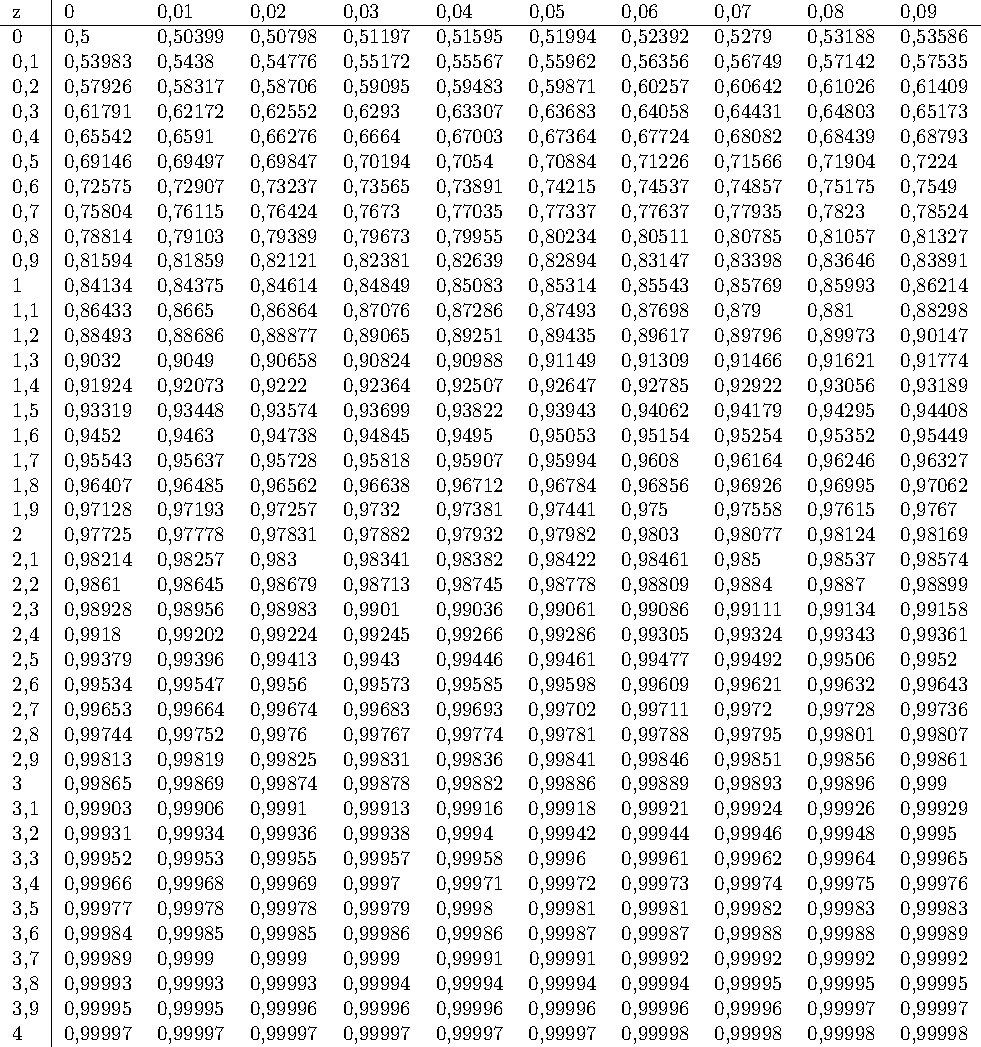
\includepdf[pages=-, scale=0.9]{distribucion_normal.pdf}

%\documentclass{article}
%\usepackage{pgfplots}
%\begin{document}



\begin{tikzpicture}

\pgfmathdeclarefunction{gauss}{2}{%
  \pgfmathparse{1/(#2*sqrt(2*pi))*exp(-((x-#1)^2)/(2*#2^2))}%
}

\begin{axis}[
  no markers, domain=0:10, samples=100,
  axis lines*=left, xlabel=$x$, ylabel=$y$,
  every axis y label/.style={at=(current axis.above origin),anchor=south},
  every axis x label/.style={at=(current axis.right of origin),anchor=west},
  height=5cm, width=12cm,
  xtick={4,6.5}, ytick=\empty,
  enlargelimits=false, clip=false, axis on top,
  grid = major
  ]
  \addplot [fill=cyan!20, draw=none, domain=0:5.96] {gauss(6.5,1)} \closedcycle;
  \addplot [very thick,cyan!50!black] {gauss(4,1)};
  \addplot [very thick,cyan!50!black] {gauss(6.5,1)};


\draw [yshift=-0.6cm, latex-latex](axis cs:4,0) -- node [fill=white] {$1.96\sigma$} (axis cs:5.96,0);
\end{axis}

\end{tikzpicture}

%\end{document}











\chapter{Inferencia estadística}
\section{Inferencia Estadística}

\paragraph{Objetivo:} Obtener conclusiones válidas para toda la población a partir del estudio de una muestra.  

\paragraph{¿Cómo?:} Mediante los métodos de estimación puntual y de intervalos de confianza

\section{Estimación puntual} Se recurre a cálculos con los datos de la muestra para inferir algunos aspectos de la población. Al cálculo realizado se le llama estadístico.

\paragraph{Definición:} Dado $\lambda$, un parámetro de la población. Decimos que el estadístico $\widehat{\lambda}$
es un estimador suyo si es
un parámetro obtenido a partir de una muestra y cuyo es asignar un valor
aproximado a $\lambda$.

La estimación puntual sirve de poco mientras
desconozcamos cuál es el grado de aproximación del estimador al parámetro real. Por ese motivo se procede
a la estimación mediante un intervalo.

\section{Estimación por intervalos de confianza} 

 A partir de una muestra aleatoria de tamaño $n$, podemos estimar el valor de un parámetro de la población del siguiente modo:
 
\begin{itemize}
\item Dando un intervalo dentro del cual confiamos que esté el parámetro. Se llama \textbf{intervalo de confianza}.
\item Hallando la probabilidad de que tal cosa ocurra. A dicha probabilidad se la llama \textbf{nivel de confianza}.
\end{itemize}


\subsection{Estimación de la media por intervalo de confianza} Se desea estimar la media, $\mu$, de una población cuya desviación típica, $\sigma$, es
conocida.
Para ello, se recurre a una muestra de tamaño n de la cual se obtiene la media,
$\overline{x}$ (media muestral).
Si la población de partida es normal, o si el tamaño de la muestra es $n \geqslant 30 $, el intervalo de confianza de $\mu$, con un nivel de confianza de $\left( 1 - \alpha \right)\cdot 100 \% $, es: $$ \left( \overline{x} - z_{\alpha / 2}\cdot \frac{\sigma}{\sqrt{n}} ,  \overline{x} + z_{\alpha / 2}\cdot \frac{\sigma}{\sqrt{n}}
\right)$$

siendo: \begin{itemize}
\item $\overline{x}$: La media de los datos de la muestra
\item $z_{\alpha / 2}$: El valor de la distribución normal $Z\leadsto N\left((0,1\right)$
\item $\sigma$: La desviación típica de la distribución de la población (o si no se conoce de un estimador sesgado de la misma)
\item $n$: El tamaño de la muestra
\end{itemize}

\paragraph{Error máximo cometido:} $$E=z_{\alpha / 2}\cdot \frac{\sigma}{\sqrt{n}}$$
Es el radio del entorno dado por el intervalo de confianza. \textbf{NOTA:} Disminuye al aumentar el tamaño de la muestra y por tanto si se quiere garantizar un error determinado para un nivel de confianza habrá que tomar muestras de al menos un \textbf{tamaño determinado de la muestra}. 

\paragraph{Ejemplo 2:} Se desea realizar una investigación para estimar el peso medio de los recién nacidos de madres fumadoras. Se admite un error máximo de 50 gramos, con una confianza del 95\%. Si por estudios anteriores se sabe que la desviación típica del peso medio de tales recién nacidos es de 400 gramos, ¿qué tamaño mínimo de muestra se necesita en la investigación?\\

\subparagraph{Solución:}$E=50$, Confianza=$95$ y $\sigma=400$ \\
$\alpha=1-0.95=0.05 \to \frac{\alpha}{2}=\frac{0.05}{2}=0.025$
. \\ Por tanto, el valor crítico será: \\
$P\left(Z \leqslant z_{\alpha / 2} \right)= 0.95 + 0.025 = 0.975 \to z_{\alpha / 2} = 1.96$\\ A partir de la definición de error máximo admitido:
$$E=z_{\alpha / 2}\cdot \frac{\sigma}{\sqrt{n}} \to 
n = \left( \frac{z_{\alpha / 2} \cdot \sigma}{E} \right) ^ 2$$
Luego: \\
$$n = \left( \frac{1.96 \cdot 400}{50} \right) ^ 2\approx 245.8534 \to n=246
$$

\subsection{Estimación de la proporción por intervalo de confianza} Se desea estimar la proporción, $p$, que una determinada característica se cumple en una población.
Para ello, se recurre a una muestra de tamaño n de la cual se calcula la 
$\overline{p}$ (proporción muestral).
Si la población de partida es normal, o si el tamaño de la muestra es $n \geqslant 30 $, el intervalo de confianza de $p$, con un nivel de confianza de $\left( 1 - \alpha \right)\cdot 100 \% $, es: $$ \left( \overline{p} - z_{\alpha / 2}\cdot \sqrt{\frac{\overline{p}\cdot\left(1-\overline{p} \right)}{n}} ,  \overline{p} + z_{\alpha / 2}\cdot \sqrt{\frac{\overline{p}\cdot\left(1-\overline{p} \right)}{n}}\right)$$

En este caso el error máximo admitido es:

$$E=z_{\alpha / 2}\cdot \sqrt{\frac{\overline{p}\cdot\left(1-\overline{p} \right)}{n}}$$

\paragraph{Ejemplo:} Para estimar la proporción de personas con sobrepeso en una población se ha tomado una
muestra aleatoria simple de tamaño 100 personas, de las cuales 21 tienen sobrepeso. Calcular el intervalo
de confianza al 96\% para la proporción de personas con sobrepeso en la población.

\subparagraph{Solución:}$\overline{p}=0.21$, Confianza=$96$ \\
$\alpha=1-0.96=0.04 \to \frac{\alpha}{2}=\frac{0.04}{2}=0.02$
. \\ Por tanto, el valor crítico será: \\

$P\left(Z \leqslant z_{\alpha / 2} \right)= 0.96 + 0.02 = 0.98 \to z_{\alpha / 2} \approx 2.05$
%\documentclass{article}
%\usepackage{pgfplots}
%\usetikzlibrary{math}
%\begin{document}



\begin{tikzpicture}[scale=0.45]

\pgfmathdeclarefunction{gauss}{2}{%
  \pgfmathparse{1/(#2*sqrt(2*pi))*exp(-((x-#1)^2)/(2*#2^2))}%
}

\tikzmath{
			\conf = 0.96; \crit= 2.05; \a=round((1-\conf)/2),2);
          }

%\begin{axis}[
%  no markers, domain=0:10, samples=100,
%  axis lines*=left, xlabel=$x$, ylabel=$y$,
%  every axis y label/.style={at=(current axis.above origin),anchor=south},
%  every axis x label/.style={at=(current axis.right of origin),anchor=west},
%  height=5cm, width=12cm,
%  xtick={4,6.5}, ytick=\empty,
%  enlargelimits=false, clip=false, axis on top,
%  grid = major
%  ]
%  \addplot [fill=cyan!20, draw=none, domain=0:5.96] {gauss(6.5,1)} \closedcycle;
%  \addplot [very thick,cyan!50!black] {gauss(4,1)};
%  \addplot [very thick,cyan!50!black] {gauss(6.5,1)};
%
%
%%\draw [yshift=-0.6cm, latex-latex](axis cs:4,0) -- node [fill=white] {$1.96\sigma$} (axis cs:5.96,0);
%\end{axis}

\begin{axis}[
  no markers, domain=-5:5, samples=100,
  axis lines=left, 
  %xlabel=$xa$, ylabel=$ya$,
  %every axis y label/.style={at=(current axis.above origin),anchor=south},
  %every axis x label/.style={at=(current axis.right of origin),anchor=west},
  height=5cm, width=12cm,
  xtick={0,\crit}, ytick=\empty,
  xticklabels = {$0$, $z_{\frac{\alpha}{2}}=\crit$},
  enlargelimits=false, clip=false, axis on top,
  %grid = major
  ]
  \addplot [fill=cyan!20, draw=none, domain=-\crit:\crit] {gauss(0,1)} \closedcycle;
  \addplot [very thick,cyan!50!black] {gauss(0,1)};
  %\addplot [very thick,cyan!50!black] {gauss(6.5,1)};
  


%\draw [yshift=-0.6cm, latex-latex](axis cs:4,0) -- node [fill=white] {$1.96\sigma$} (axis cs:5.96,0);
\end{axis}
\node[] at (5.2,1.5) {$\conf$};	
\draw[->]   (\crit+6.5,1)node[right]{$\a$}  --  (\crit+5.6,0.1) ;



\end{tikzpicture}

%\end{document} 
A partir de la definición de error máximo admitido:
$$E=z_{\alpha / 2}\cdot \sqrt{\frac{\overline{p}\cdot\left(1-\overline{p} \right)}{n}}\approx 2.05 \cdot \sqrt{\frac{0.21\cdot 0.79}{100}}\approx 0.08$$
Luego el intervalo es: \\ 
$$\left( 0.21 - 0.08 , 0.21 + 0,08 \right) = \left(0.13, 0.29 \right)
$$
Por tanto con una alta probabilidad, en concreto 0.96, el porcentaje de individuos con sobrepeso en la población se encuentra entre el 13\% y el 29\% 

\subsection{Conclusiones} A ver







\chapter{Miscelánea}
%% Options for packages loaded elsewhere
%\PassOptionsToPackage{unicode=true}{hyperref}
%\PassOptionsToPackage{hyphens}{url}
%%
%\documentclass[
%]{article}
%\usepackage{lmodern}
%\usepackage{amssymb,amsmath}
%\usepackage{ifxetex,ifluatex}
%\ifnum 0\ifxetex 1\fi\ifluatex 1\fi=0 % if pdftex
%  \usepackage[T1]{fontenc}
%  \usepackage[utf8]{inputenc}
%  \usepackage{textcomp} % provides euro and other symbols
%\else % if luatex or xelatex
%  \usepackage{unicode-math}
%  \defaultfontfeatures{Scale=MatchLowercase}
%  \defaultfontfeatures[\rmfamily]{Ligatures=TeX,Scale=1}
%\fi
%% Use upquote if available, for straight quotes in verbatim environments
%\IfFileExists{upquote.sty}{\usepackage{upquote}}{}
%\IfFileExists{microtype.sty}{% use microtype if available
%  \usepackage[]{microtype}
%  \UseMicrotypeSet[protrusion]{basicmath} % disable protrusion for tt fonts
%}{}
%\makeatletter
%\@ifundefined{KOMAClassName}{% if non-KOMA class
%  \IfFileExists{parskip.sty}{%
%    \usepackage{parskip}
%  }{% else
%    \setlength{\parindent}{0pt}
%    \setlength{\parskip}{6pt plus 2pt minus 1pt}}
%}{% if KOMA class
%  \KOMAoptions{parskip=half}}
%\makeatother
%\usepackage{xcolor}
%\IfFileExists{xurl.sty}{\usepackage{xurl}}{} % add URL line breaks if available
%\IfFileExists{bookmark.sty}{\usepackage{bookmark}}{\usepackage{hyperref}}
%\hypersetup{
%  hidelinks,
%}
%\urlstyle{same} % disable monospaced font for URLs
%\setlength{\emergencystretch}{3em} % prevent overfull lines
%\providecommand{\tightlist}{%
%  \setlength{\itemsep}{0pt}\setlength{\parskip}{0pt}}
%\setcounter{secnumdepth}{-\maxdimen} % remove section numbering
%% Redefines (sub)paragraphs to behave more like sections
%\ifx\paragraph\undefined\else
%  \let\oldparagraph\paragraph
%  \renewcommand{\paragraph}[1]{\oldparagraph{#1}\mbox{}}
%\fi
%\ifx\subparagraph\undefined\else
%  \let\oldsubparagraph\subparagraph
%  \renewcommand{\subparagraph}[1]{\oldsubparagraph{#1}\mbox{}}
%\fi
%
%% Set default figure placement to htbp
%\makeatletter
%\def\fps@figure{htbp}
%\makeatother
%
%
%\date{}
%
%\begin{document}
%

\definecolor{wrwrwr}{rgb}{0.3803921568627451,0.3803921568627451,0.3803921568627451}
\definecolor{rvwvcq}{rgb}{0.08235294117647059,0.396078431372549,0.7529411764705882}

\hypertarget{rectas-y-puntos-notables-de-un-triuxe1ngulo}{%
\section{Rectas y puntos notables de un
triángulo}\label{rectas-y-puntos-notables-de-un-triuxe1ngulo}}

\hypertarget{mediana}{%
\subsection{Mediana}\label{mediana}}

La \textbf{mediana} es el segmento que va del punto medio de un lado al
vértice opuesto.

Al punto dónde se cortan las medianas de un triángulo se le llama
\textbf{baricentro} y constituye el centro de gravedad del polígono.

%
%\documentclass[10pt]{standalone}
%\usepackage{pgf,tikz,pgfplots}
%\pgfplotsset{compat=1.15}
%\usepackage{mathrsfs}
%\usetikzlibrary{arrows}
%%\pagestyle{empty}
%
%\begin{document}
%% Medianas y baricentro
%
%\definecolor{wrwrwr}{rgb}{0.3803921568627451,0.3803921568627451,0.3803921568627451}
%\definecolor{rvwvcq}{rgb}{0.08235294117647059,0.396078431372549,0.7529411764705882}
\begin{tikzpicture}[line cap=round,line join=round,>=triangle 45,scale=0.65]
\clip(-6.154568000000002,-1.8982211062725844) rectangle (4.106232000000003,7.1694626146576494);
\fill[line width=2pt,color=rvwvcq,fill=rvwvcq,fill opacity=0.10000000149011612] (-5,-1) -- (3,-1) -- (0,6) -- cycle;
\draw [line width=2pt,color=rvwvcq] (-5,-1)-- (3,-1);
\draw [line width=2pt,color=rvwvcq] (3,-1)-- (0,6);
\draw [line width=2pt,color=rvwvcq] (0,6)-- (-5,-1);
\draw [line width=2pt,color=wrwrwr] (-2.5,2.5)-- (3,-1);
\draw [line width=2pt,color=wrwrwr] (-1,-1)-- (0,6);
\draw [line width=2pt,color=wrwrwr] (-5,-1)-- (1.5,2.5);
\begin{scriptsize}
\draw [fill=rvwvcq] (-5,-1) circle (2.5pt);
\draw[color=rvwvcq] (-4.911871111111114,-0.7361607091015785) node {$A$};
\draw [fill=rvwvcq] (3,-1) circle (2.5pt);
\draw[color=rvwvcq] (3.091552888888891,-0.7361607091015785) node {$B$};
\draw [fill=rvwvcq] (0,6) circle (2.5pt);
\draw[color=rvwvcq] (0.09311911111111175,6.260285827233702) node {$C$};
\draw [fill=wrwrwr] (-1,-1) circle (2pt);
\draw[color=wrwrwr] (-0.9101591111111109,-0.7602448624108221) node {$D$};
\draw [fill=wrwrwr] (-2.5,2.5) circle (2pt);
\draw[color=wrwrwr] (-2.403675555555556,2.731957367429507) node {$E$};
\draw [fill=wrwrwr] (1.5,2.5) circle (2pt);
\draw[color=wrwrwr] (1.586635555555557,2.731957367429507) node {$F$};
\draw [fill=wrwrwr] (-0.6666666666666666,1.3333333333333333) circle (2pt);
\draw[color=wrwrwr] (0.6843262222222229,1.359160628802619) node {$Baricentro$};
\end{scriptsize}
\end{tikzpicture}
%\end{document}

\hypertarget{mediatriz}{%
\subsection{Mediatriz}\label{mediatriz}}

La \textbf{mediatriz} de un segmento es la recta perpendicular al punto medio.
Geométricamente son los puntos del plano que equidistan a ambos extremos
del segmento.

En un triángulo llamaremos mediatriz a la mediatriz de cada uno de los
lados.

El punto de corte de las tres mediatrices equidista a los tres vértices
del triángulo. Ha dicho punto se le llama \textbf{circuncentro} porque permite
circunscribir el triángulo en una circunferencia de centro dicho punto.

%\documentclass[10pt]{article}
%\usepackage{pgf,tikz,pgfplots}
%\pgfplotsset{compat=1.15}
%\usepackage{mathrsfs}
%\usetikzlibrary{arrows}
%\pagestyle{empty}
%\begin{document}
%\definecolor{wrwrwr}{rgb}{0.3803921568627451,0.3803921568627451,0.3803921568627451}
%\definecolor{rvwvcq}{rgb}{0.08235294117647059,0.396078431372549,0.7529411764705882}
\begin{tikzpicture}[grow=right, sloped, scale=0.7]\clip(-6.154568000000002,-3.8982211062725844) rectangle (4.2,7);
\fill[line width=2pt,color=rvwvcq,fill=rvwvcq,fill opacity=0.10000000149011612] (-5,-1) -- (3,-1) -- (0,6) -- cycle;
\draw [line width=2pt,color=rvwvcq] (-5,-1)-- (3,-1);
\draw [line width=2pt,color=rvwvcq] (3,-1)-- (0,6);
\draw [line width=2pt,color=rvwvcq] (0,6)-- (-5,-1);
\draw [line width=2pt,color=wrwrwr] (-1,-6.399108752051755) -- (-1,9.599938859846416);
\draw [line width=2pt,color=wrwrwr,domain=-13.636070873907869:13.273820660511266] plot(\x,{(--5-5*\x)/7});
\draw [line width=2pt,color=wrwrwr,domain=-13.636070873907869:13.273820660511266] plot(\x,{(-13-3*\x)/-7});
\draw [line width=2pt,color=wrwrwr] (-1,1.4285714285714286) circle (4.679525529759771cm);
\begin{scriptsize}
\draw [fill=rvwvcq] (-5,-1) circle (2.5pt);
\draw[color=rvwvcq] (-4.808111733768611,-0.46196217732391776) node {$A$};
\draw [fill=rvwvcq] (3,-1) circle (2.5pt);
\draw[color=rvwvcq] (3.191486629145785,-0.46196217732391776) node {$B$};
\draw [fill=rvwvcq] (0,6) circle (2.5pt);
\draw[color=rvwvcq] (0.18572038035842364,6.537621152881533) node {$C$};
\draw [fill=wrwrwr] (-1,-1) circle (2pt);
\draw[color=wrwrwr] (-0.8083125523114124,-0.5119592011110996) node {$D$};
\draw [fill=wrwrwr] (-2.5,2.5) circle (2pt);
\draw[color=wrwrwr] (-2.2993619513161665,2.9878324639916256) node {$E$};
\draw [fill=wrwrwr] (1.5,2.5) circle (2pt);
\draw[color=wrwrwr] (1.700437230141031,2.9878324639916256) node {$F$};
\draw [fill=wrwrwr] (-1,1.4285714285714286) circle (2pt);
\draw[color=wrwrwr] (1.1797533130282598,1.3129321671210357) node {$Circuncentro$};
\end{scriptsize}
\end{tikzpicture}
%\end{document}

\hypertarget{altura}{%
\subsection{Altura}\label{altura}}

Llamaremos \textbf{altura} de un triángulo al segmento perpendicular a un lado y
pasa por el vértice opuesto.

Al punto de corte de las alturas se le llama \textbf{ortocentro}.

%\documentclass[10pt]{article}
%\usepackage{pgf,tikz,pgfplots}
%%\pgfplotsset{compat=1.15}
%\usepackage{mathrsfs}
%\usetikzlibrary{arrows}
%\pagestyle{empty}
%\newcommand{\degre}{\ensuremath{^\circ}}
%\begin{document}
%\definecolor{wrwrwr}{rgb}{0.3803921568627451,0.3803921568627451,0.3803921568627451}
%\definecolor{rvwvcq}{rgb}{0.98235294117647059,0.396078431372549,0.7529411764705882}
\begin{tikzpicture}[grow=right, sloped, scale=0.7]\clip(-6.154568000000002,-3.8982211062725844) rectangle (4.2,7);
\clip(-11.145015598814782,-9.076966577456616) rectangle (18.28831648795786,8.422371196936597);
\fill[line width=2pt,color=rvwvcq,fill=rvwvcq,fill opacity=0.10000000149011612] (-5,-1) -- (3,-1) -- (0,6) -- cycle;
\draw[line width=1.6pt,fill=black,fill opacity=0.10000000149011612] (-2.616480014189626,2.336927980134524) -- (-2.1696242105403662,2.0177452632421953) -- (-1.8504414936480373,2.464601066891455) -- (-2.2972972972972974,2.7837837837837838) -- cycle; 
\draw[line width=1.6pt,fill=black,fill opacity=0.10000000149011612] (1.5423027784864105,2.401293516865042) -- (1.0375609857592993,2.1849756056962804) -- (1.2538788969280612,1.6802338129691692) -- (1.7586206896551724,1.896551724137931) -- cycle; 
\draw[line width=1.6pt,fill=black,fill opacity=0.10000000149011612] (0.5491427100652383,-1) -- (0.5491427100652384,-0.4508572899347618) -- (0,-0.4508572899347617) -- (0,-1) -- cycle; 
\draw [line width=2pt,color=rvwvcq] (-5,-1)-- (3,-1);
\draw [line width=2pt,color=rvwvcq] (3,-1)-- (0,6);
\draw [line width=2pt,color=rvwvcq] (0,6)-- (-5,-1);
\draw [line width=2pt,color=wrwrwr] (0,-9.076966577456616) -- (0,8.422371196936597);
\draw [line width=2pt,color=wrwrwr,domain=-11.145015598814782:18.28831648795786] plot(\x,{(-8-3*\x)/-7});
\draw [line width=2pt,color=wrwrwr,domain=-11.145015598814782:18.28831648795786] plot(\x,{(--8-5*\x)/7});
\begin{scriptsize}
\draw [fill=rvwvcq] (-5,-1) circle (2.5pt);
\draw[color=rvwvcq] (-4.802740874752074,-0.42299719371372185) node {$A$};
\draw [fill=rvwvcq] (3,-1) circle (2.5pt);
\draw[color=rvwvcq] (3.1962913282494623,-0.42299719371372185) node {$B$};
\draw [fill=rvwvcq] (0,6) circle (2.5pt);
\draw[color=rvwvcq] (0.21930523328125284,6.576737916043563) node {$C$};
\draw[color=black] (-1.0750365471397076,2.530016055715133) node {$\alpha = 90\textrm{\degre}$};
\draw[color=black] (2.3937994243884666,2.256588902990239) node {$\beta = 90\textrm{\degre}$};
\draw[color=black] (1.4877601780937941,-0.4776826242587007) node {$\gamma = 90\textrm{\degre}$};
\draw [fill=wrwrwr] (0,1.1428571428571428) circle (2pt);
\draw[color=wrwrwr] (1.8501758766116632,1.1355375768181737) node {$Ortocentro$};
\end{scriptsize}
\end{tikzpicture}
%\end{document}

\hypertarget{bisectriz}{%
\subsection{Bisectriz}\label{bisectriz}}

Llamamos \textbf{bisectriz} de un ángulo a la semirrecta que divide al ángulo en
dos ángulos iguales.
En un triángulo tendremos las tres bisectrices correspondientes a cada uno de los tres ángulos.

Llamaremos \textbf{incentro} al punto de corte de las bisectrices de un triángulo.

%\documentclass[10pt]{article}
%\usepackage{pgf,tikz,pgfplots}
%\pgfplotsset{compat=1.15}
%\usepackage{mathrsfs}
%\usetikzlibrary{arrows}
%\pagestyle{empty}
%\newcommand{\degre}{\ensuremath{^\circ}}
%\begin{document}
%\definecolor{wrwrwr}{rgb}{0.3803921568627451,0.3803921568627451,0.3803921568627451}
%\definecolor{rvwvcq}{rgb}{0.08235294117647059,0.396078431372549,0.7529411764705882}
\begin{tikzpicture}[grow=right, sloped, scale=0.6]\clip(-6.154568000000002,-3.8982211062725844) rectangle (4.2,7);
\fill[line width=2pt,color=rvwvcq,fill=rvwvcq,fill opacity=0.10000000149011612] (-5,-1) -- (3,-1) -- (0,6) -- cycle;
\draw [shift={(0,6)},line width=1.6pt,fill=black,fill opacity=0.10000000149011612] (0,0) -- (-125.53767779197437:0.7766050682525762) arc (-125.53767779197437:-66.8014094863518:0.7766050682525762) -- cycle;
\draw [shift={(-5,-1)},line width=1.6pt,fill=black,fill opacity=0.10000000149011612] (0,0) -- (0:0.7766050682525762) arc (0:54.462322208025626:0.7766050682525762) -- cycle;
\draw [shift={(3,-1)},line width=1.6pt,fill=black,fill opacity=0.10000000149011612] (0,0) -- (113.19859051364813:0.7766050682525762) arc (113.19859051364813:180:0.7766050682525762) -- cycle;
\draw [shift={(3,-1)},line width=1.6pt,fill=black,fill opacity=0.10000000149011612] (0,0) -- (113.19859051364813:0.7766050682525762) arc (113.19859051364813:146.59929525682406:0.7766050682525762) -- cycle;
\draw [shift={(0,6)},line width=1.6pt,fill=black,fill opacity=0.10000000149011612] (0,0) -- (-125.53767779197437:0.7766050682525762) arc (-125.53767779197437:-96.1695436391631:0.7766050682525762) -- cycle;
\draw [shift={(-5,-1)},line width=1.6pt,fill=black,fill opacity=0.10000000149011612] (0,0) -- (0:0.7766050682525762) arc (0:27.231161104012813:0.7766050682525762) -- cycle;
\draw [line width=2pt,color=rvwvcq] (-5,-1)-- (3,-1);
\draw [line width=2pt,color=rvwvcq] (3,-1)-- (0,6);
\draw [line width=2pt,color=rvwvcq] (0,6)-- (-5,-1);
\draw [line width=2pt,color=wrwrwr,domain=-13.604264981614604:15.829067105158035] plot(\x,{(-0.8166319340003523--0.5504910087462067*\x)/-0.8348410922382679});
\draw [line width=2pt,color=wrwrwr,domain=-13.604264981614604:15.829067105158035] plot(\x,{(-0.6448253150018926-0.9942082320611364*\x)/-0.10747088583364875});
\draw [line width=2pt,color=wrwrwr,domain=-13.604264981614604:15.829067105158035] plot(\x,{(--1.3987402615700915--0.4575815808579403*\x)/0.88916764271961});
\draw [line width=2pt,color=wrwrwr] (-0.5067239194106411,1.3123202795579019) circle (2.313929526200274cm);
\begin{scriptsize}
\draw [fill=rvwvcq] (-5,-1) circle (2.5pt);
\draw[color=rvwvcq] (-4.8027408747520735,-0.42299719371372047) node {$A$};
\draw [fill=rvwvcq] (3,-1) circle (2.5pt);
\draw[color=rvwvcq] (3.196291328249462,-0.42299719371372047) node {$B$};
\draw [fill=rvwvcq] (0,6) circle (2.5pt);
\draw[color=rvwvcq] (0.2193052332812528,6.576737916043568) node {$C$};
\draw[color=black] (-0.7643945198386772,5.838484603686354) node {$\alpha = 58.7\textrm{\degre}$};
\draw[color=black] (-2.498812505602764,0.2332279728260253) node {$\beta = 54.5\textrm{\degre}$};
\draw[color=black] (3.222178163857881,0.5066551255509193) node {$\gamma = 66.8\textrm{\degre}$};
\draw[color=black] (2.005496890262178,-0.5050253395311887) node {$\delta = 33.4\textrm{\degre}$};
\draw[color=black] (1.6689680273527285,5.07288857605665) node {$\epsilon = 29.4\textrm{\degre}$};
\draw[color=black] (-2.265830985126991,-0.47768262425869923) node {$\zeta = 27.2\textrm{\degre}$};
\draw [fill=wrwrwr] (-0.5067239194106411,1.3123202795579019) circle (2pt);
\draw[color=wrwrwr] (-0.5572998349713234,0.42462697973345115) node {$Incentro$};
\draw [fill=wrwrwr] (-2.438487372426055,2.5861176786035225) circle (2pt);
\draw[color=wrwrwr] (-2.239944149518572,3.131555791709902) node {$D$};
\end{scriptsize}
\end{tikzpicture}
%\end{document}

%\end{document}



\end{document}
